% simple.tex - simple Master's thesis sample
% $Id: simple.tex 309 2011-01-28 14:46:48Z vlado $
%\documentclass[12pt]{dalcsthesis}
% to prepare draft version use option draft:
\documentclass[12pt,draft]{dalcsthesis}
\usepackage{verbatim}
\usepackage{amsmath}
\usepackage{amssymb}
\usepackage{adjustbox}
\usepackage{tabularx}
\usepackage{subfigure}
\usepackage{algorithm2e}

%\usepackage{caption}
%\captionsetup[table]{skip=10pt}
\usepackage{graphicx}
\usepackage{epstopdf}
\begin{document}
\mcs  % options are \mcs, \macs, \mec, \mhi, \phd, and \bcshon
\title{Feature Based adaptive motion model}
\author{Rohan Bhargava}
\defenceday{1}
\defencemonth{October}
\defenceyear{2013}
\convocation{January}{2014}

% Use multiple \supervisor commands for co-supervisors.
% Use one \reader command for each reader.

\supervisor{Dr. Thomas Trappenberg}
\supervisor{Dr. Mae Sato}
\reader{D. Odaprof}
\reader{A. External}
\providecommand{\tabularnewline}{\\}
\newcommand{\lyxdot}{.}
\nolistoftables
\nolistoffigures

\frontmatter


\begin{abstract}
We present a method to learn and adapt the motion model. The motion model can be influenced by environmental properties and is a crucial part of the navigation system.Examples are the drift that is accounted in the motion model can be different for carpets and tiles. The AUV can have a change in their motion model when they are moving from fresh water to sea water. Our algorithm is based on the Expectation Maximization Framework which help us to learn the right parameters for the model.
The Expectation Step is completed by particle filtering and smoothing. The Maximization step involves finding the parameters for the model.We use side sonar images to extract landmarks which can gives us position estimates to help us evolve our motion model.This leads to a better position estimate of the robot. 
We found that the our learning motion model adapted well to the change in parameters and had low localization error compared to static motion model. 
This algorithm eliminates the need for laborious and hand-tuning calibration process. The main significance of learning the motion model is to have better navigation algorithms and also its a step towards robots being able to adapt to environment without human intervention.
We validate our approach by recovering a good motion model when the density,temperature of the water is changed in our simulations. 
\end{abstract}

\begin{acknowledgements}
Thanks to all the little people who make me look tall.
\end{acknowledgements}

\mainmatter

\chapter{Introduction}
 





\section{Motivation}
The core of human environment interaction is the ability of a person to know its position in surrounding environment. The process of estimating the robot’s position and orientation in the world is termed as Localization \cite{thrun2005probabilistic}.  A common approach to determine the location of a robot is through the use of Global Positioning System (GPS), a segries of satellites in low earth orbit that use differential positioning to determine a location for a receiver.  Another approach is to provide a prior map of the environment and with help of sensors a robot perceives the world and localizes itself in it. An additional challenge to the localization is when sensing of the external environment is impossible or incomplete due to unreliability and inaccessibility of the sensors. In this case the localization estimate can be updated using self-generated cues such as acceleration and velocity.  

An example for such a scenario from underwater robotics is maintaining a pose estimate of an Autonomous Underwater Vehicle, such as Hugin 4500 (Figure ~\ref{fig-Hugin 4500}). In AUV the pose estimation relies on Inertial Navigation Systems (INS) which gives an estimate of the velocity, position and orientation.  All INS systems suffer from drift i.e. small errors in measurement of acceleration and angular velocity are integrated into progressively larger error.  To compensate for the drift systems such as Doppler Velocity Log (DVL), surface GPS etc. are used \cite{Lammas2004} \cite{leonard1998autonomous}. Hegrenaes et al \cite{Hegrenes2008} pointed out that there are situations where these systems fail or readings from these sensors need to be discarded due to poor quality.  An example of such a situation is the non-feasibility of the vehicle to surface.  In such situations they proposed to use the self-generated velocity estimates to aid INS systems. 
\begin{figure}
  \centering
     {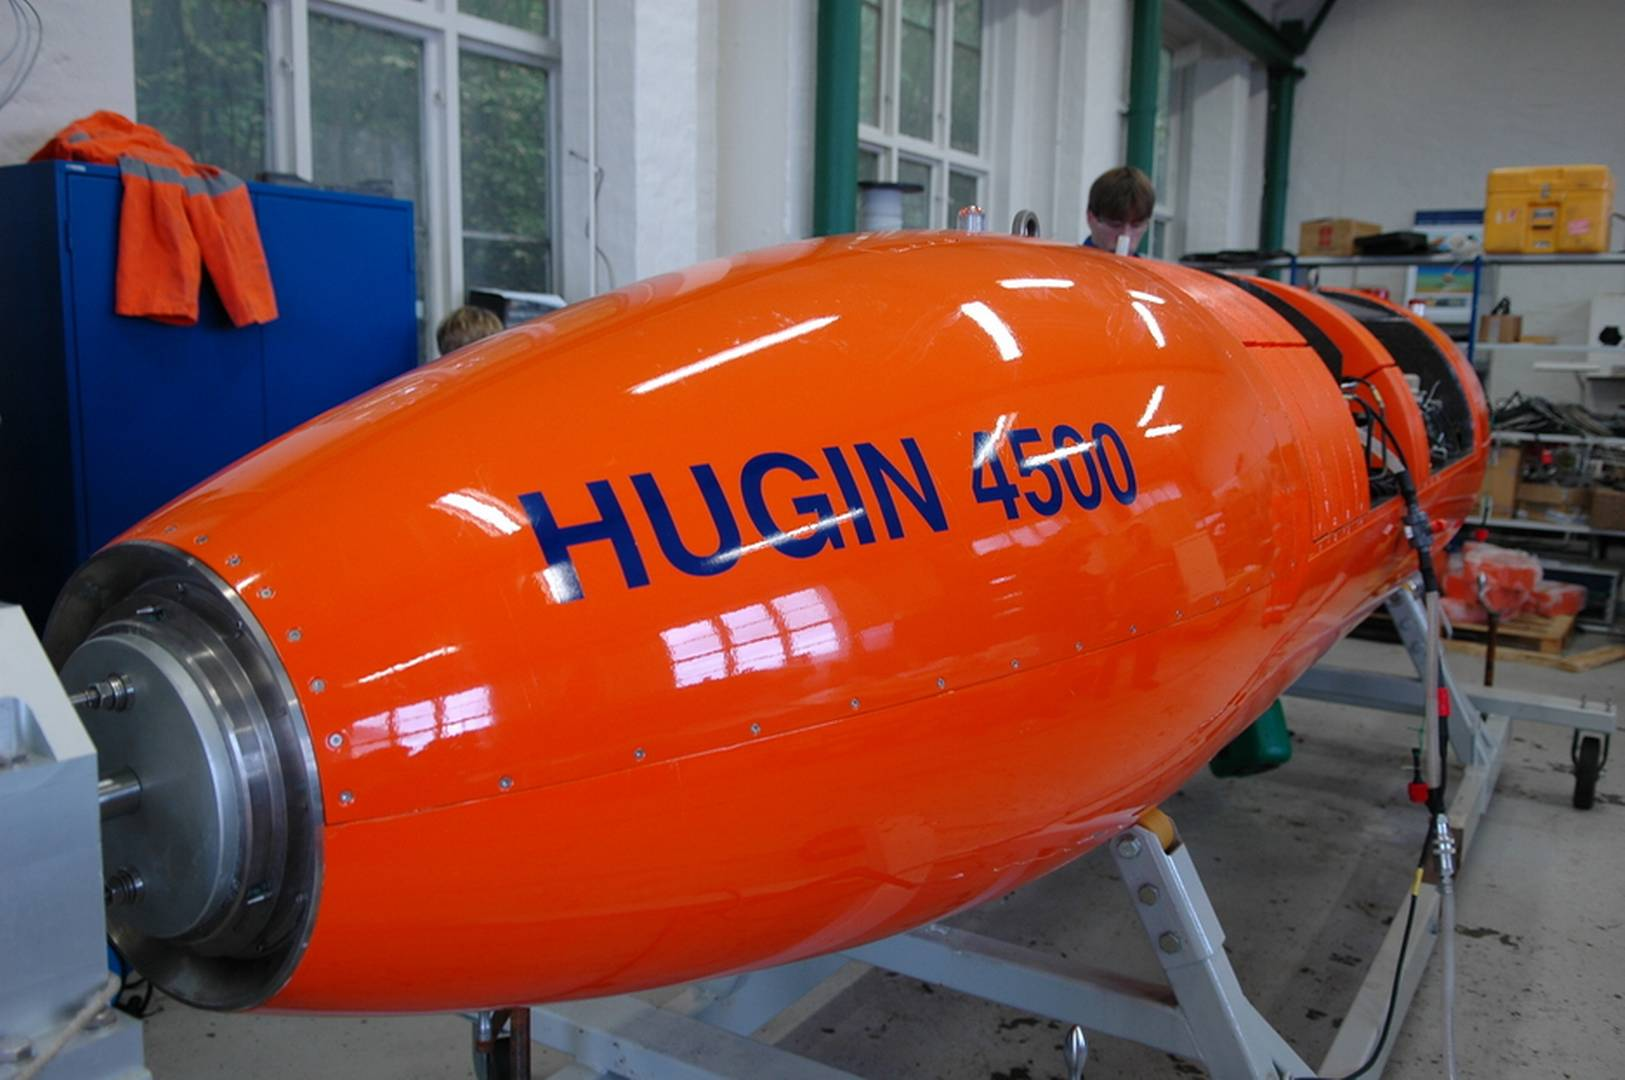
\includegraphics[height = 3.0 in]{../hugin_4500.png}}
  \caption{\label{fig-Hugin 4500} Hugin 4500 autonomous underwater vehicles. When submerged, the vehicle uses dead reckoning, incorporating DVL and compass input to maintain an estimate on current positioning.
}
\end{figure}


The estimates can be difficult to acquire and maintain due to uncertainties in way a robot interacts and senses its environment. These uncertainties can arise due to noisy and incomplete sensing of the environment, uncertain movements of a robot in the environment and changes in the environment itself.  To address these issues Sebastian Thrun \cite{thrun2005probabilistic} represented the motion and sensor models probabilistically. He defines it as instead of relying on single “best guess” as to what might be the case, probabilistic algorithms represent the information by probability distributions over a whole space of guesses.  To update the state of a robot probabilistically there are algorithms such as Kalman Filter \cite{kalman1960new}, Particle Filter \cite{gordon1993novel} etc. which are based on Bayes filter. 

In probabilistic robotics the motion and sensors models are represented by a distribution which is defined by its parameters.  The process of determining parameters to kinematic model is termed as calibration \cite{cox1990autonomous} \cite{vukobratovic1989introduction}. Generally the parameters to the models are hand tuned and are derived by conducting calibration experiments. Such calibration methods are impractical for two reasons. Firstly these processes are labour intensive and require prior information about the environment and robot. Secondly, changes in robot (e.g.-:  general wear and tear) and environment (e.g.-: moving from fresh water to sea water). The changes in underwater environments can be due to change in density, temperature etc. of water. These changes require recalibration of a robot while it is in operation which in most cases is not possible to do. The inaccuracies in the models will effect results for higher level tasks such as path planning \cite{Lav06}, Simultaneous Localization and 
Mapping (SLAM) \cite{thrun2005probabilistic} \cite{grisettiyz2005improving} etc.

Roy and Thrun \cite{Roy} proposed an online calibration method for land robots which can be performed without human intervention.  They approached the calibration process as maximum likelihood estimation problem which gives an estimate of parameters for the given data. The calibration parameters are iteratively estimated by comparing pair of subsequent sensor readings. The algorithm proposed worked well for systematic drifts and the results showed the position error reduced by approximately by 83%.

Alizar and Parr \cite{Eliazar2004} continued the work further by estimating non-systematic drifts.  They proposed an algorithm to learn the right parameters of a motion model for a land robot using Expectation Maximization Framework \cite{dempster1977maximum}. It is an unsupervised machine learning technique that alternated between the expectation and maximization step. In the Expectation Step it creates an expectation of the log-likelihood using the current estimate of the parameters and the Maximization step which computes parameters maximizing the expected log-likelihood found in the Expectation Step. They were able to learn accurate motion models with very little user input.

Yapp \cite{Yap2008} took Alizar and Parr \cite{Eliazar2004} work further and proposed an algorithm to learn the motion and sensor models for land robots. They used the same Expectation Maximization framework to learn the right parameters for the models. To calculate the like trajectory of a robot both the algorithms implemented particle filtering \cite{ristic2004beyond} \cite{chen2003bayesian} and smoothing \cite{doucet2000monte}.  The algorithm started with an estimate of initial parameters and iteratively optimized the parameters based on the data collected during robot’s operation. The algorithm assumed that a prior map of the environment is provided. 

In my thesis I specifically deal with water environments such as oceans, rivers etc. which are highly dynamic.  The algorithm proposed here is different from the work done before in two ways. Firstly the algorithm is meant to learn the right parameters for an AUV’s motion model. Secondly, the algorithm can learn motion model for unknown environments by generating landmarks using side sonar images and therefor doesn’t have to rely on static maps. Sound Navigation and Ranging (SONAR) is a technique based on sound propagation used for detecting objects underwater. Side scan sonar is a specific type of sonar used to image the topography of a sea floor.  The SONAR sensor is the only imaging tool that can work at high depth. 

My algorithm uses EM algorithm to calculate the most likely parameters for a data set.  The trajectories are calculated by implementing particle filtering and smoothing.  Particle Filters are chosen because they can mode non-linear transformations as well as have no restrictions in model. Particle smoothing was performed because Russel and Norving [refer] pointed out that the state of the system is better estimated by smoothing as it incorporates more information that just filtering. 

The remainder of the thesis is structured as follows. Chapter 2 will explain the motion model for AUV as well as give an insight on particle filtering and smoothing. Chapter 3 will give an overview of Expectation Maximization and show how this framework is used to adapt parameters for a motion model. Chapter 4 will give explain how landmarks are extracted from side sonar images. The reliability of the landmarks are shown by extracting motion information and the algorithm to do that is described in Chapter 4. Chapter 5 consist results of a simulated experiment to show the effectiveness of the algorithm. This chapter also includes the comparison of motion estimation using side sonar images to DVL.
 
\begin{comment}
 The core of human environment interaction is the ability of a person to know its position in surrounding environment. The process of estimating robot's position and orientation in the world is termed as Localization \cite{thrun2005probabilistic}. It is the answer to the question “Where am I?”. The current location of a robot can be determined by Global Positioning Systems, landmarks, maps etc. A common approach is to provide a prior map of the environment and a robot with help of sensors perceives the world and localizes itself in it. Another way to estimate the position of a robot is by knowing how a robot moves in the world . For example by knowing at what velocity a robot is moving we can predict its future location. There are various algorithms such as Particle Filter \cite{gordon1993novel},Kalman Fitler \cite{kalman1960new} etc. to estimate the state of a robot. The way the robot moves and senses the world are captured in motion and sensor models. These models are basic building blocks to various 
algorithms such as path planning \cite{Lav06}, Simultaneous Localization and Mapping (SLAM) \cite{thrun2005probabilistic} \cite{grisettiyz2005improving}  etc. which require an accurate estimate of robot's position. 

In order to account for the uncertainty in motion Sebastian Thrun \cite{thrun2005probabilistic} represented the models probabilistically. Eliazar and Parr \cite{Eliazar2004} pointed out that the essential input are the parameters to these models. The process of determining the parameters to a kinematic model is termed as calibration. Generally the robot is calibrated at the start of the experiment and the parameter values are not changed throughout the experiment. In practice wherever there is a significant change in the environment, robots are manually re calibrated during the experiment. In most of the cases it is not possible to recalibrate while the robot is in operation. As our environments are dynamic our models need to adapt to them. Eliazar and Parr \cite{Eliazar2004} proposed an algorithm to learn parameters of a motion model for land robots. Teddy Yapp \cite{Yap2008} took the work further and learned parameters for motion and sensor models for land robots. Both of their algorithms used 
Expectation Maximization framework to learn right parameters for models.

For my thesis I specifically deal with water environments such as oceans, rivers etc. which are highly dynamic and will lead to changes in motion model for Autonomous Underwater Vehicle. A specific application to demonstrate the importance of accurate motion model is Navigation. In AUV navigation relies on Inertial Navigation System(INS) which gives an estimate of velocity, position and orientation. All INS systems suffer from drift i.e. small errors in measurement of acceleration and angular velocity are integrated into progressively into larger error. Hegrenaes et al \cite{Hegrenes2008} pointed out that systems such as Doppler Velocity Log(DVL), surface GPS etc are used to compensate for the drift but they are situations where these systems fail or readings are discarded due to poor quality. To solve this particular problem they used velocity estimate from a static motion model to aid INS systems. In my thesis I propose an online system for an AUV to adapt its motion model to the dynamic environment which 
can be used for applications such as navigation as well as automate the calibration process. 

In Chapter~\ref{learning the motion model} I demonstrate how the parameters of a motion model can be estimated during its normal operation. The algorithm uses machine learning methods to learn the parameters as well as eliminate the necessity of identifying the parameters through a manual laborious calibration process. Yapp \cite{Yap2008} in his algorithm used Expectation Maximization \cite{dempster1977maximum} framework to estimate the right parameters for the model and I use the same framework for my algorithm. It is an unsupervised machine learning technique primarily used to estimate parameters. It alternates between the Expectation Step which creates an expectation of the log-likelihood using the current estimate of the parameters and the Maximization Step which computes parameters maximizing the expected log-likelihood found in the E step. 

In the algorithm proposed by Yapp \cite{Yap2008} to calculate the likely trajectory of a robot particle filtering \cite{ristic2004beyond} \cite{chen2003bayesian} and smoothing \cite{doucet2000monte} \cite{doucet2009tutorial} were performed using the sensor data collected during robot's normal operation. The particle filters were chosen because they can model non-linear transformations as well as they have no restrictions in model. Particle smoothing was performed because Russel and Norving \cite{russell2003artificial} pointed out the state of the system is better estimated by smoothing as it incorporates more information than just filtering. The maximum likelihood estimate of the parameters given the robot's trajectory and the motion data is calculated. The algorithm by Yapp \cite{Yap2008} was for land robots as well as assumed a prior map of the environment.  

The algorithm proposed in this thesis is for an AUV and can learn the motion model in unknown environments. In the algorithm instead of using a static map we used landmarks. In AUV the landmarks are extracted from side sonar images and are collected as sensor data. The algorithm assumes that the robot is equipped with a side sonar sensor and has access to its noisy motion data. Sound Navigation and Ranging (SONAR) is a technique based on sound propagation used for detecting objects underwater. The SONAR sensor is the only imaging tool which can work at high depth. Side scan sonar is a specific type of sonar used to image the topography of the sea floor.

To summarize I am proposing an algorithm to learn the right parameters of a motion model for an AUV. The parameters are learned on the fly without having a prior map or revisiting places. Results of the simulated experiment are presented in chapter ~\ref{results} to show the effectiveness of the algorithm. 
\end{comment}


 

\section{Contributions}
The main contributions of the algorithm are-:

1) \textbf{Adaptive Motion Model}-: The motion model for AUVs adapt to changing environment. This automated process of calibration of the robots lead to no hand tuning of the models and gives us an online process which can be preformed during the robot's mission.  

2) \textbf{Motion Estimation from Side Sonar Images}-: We present an approach to estimate the movement from side sonar images which can be coupled with existing motion model and can improve localization. It can be easily be performed on-board as limited amount of interest points are used which lead to lesser computation and memory usage. 

\chapter{Background}
In the chapter we start by discussing how motion models are probabilistically represented as well as give an insight about motion models for AUV. This helps us in understanding on how motion model captures the probabilistic movements of robots. We then discuss a probabilistic state estimation algorithm such as particle filter \cite{ristic2004beyond} \cite{chen2003bayesian} which is at the heart of my algorithm as well as many other robotics systems. Lastly we discuss about particle smoothing \cite{doucet2000monte} \cite{doucet2009tutorial} which gives an estimate of ground truth by calculating the distribution of past states with taking into account all the evidence up to present. 

\section{Motion Model}
\label{chap-:Motion Model}
A motion model is responsible for capturing the relationship between the control input and the change in robot's configuration. Thrun \cite{thrun2005probabilistic} models the motion of a robot probabilistically because the same
control inputs will never reproduce the same motion. A good motion model will capture the errors such as drift that are encountered during the motion of the robot. The motion model is a necessary ingredient of many algorithms such as localization,mapping etc. 

Let $X=(x,y,\theta)$ be the initial pose of the robot in x-y space. Mathematically the motion model can be described as $P(X^{'}|X,u)$, where $X^{'}$ is the pose after executing the motion command $u$. Based on the control input Thrun \cite{thrun2005probabilistic} divided the motion model in two classes 1) Odometry based motion model 2) Velocity based motion model.

The first class of motion models are used for robots equipped with wheel encoders. Odometry is generally obtained by integrating wheel encoders information and is more accurate than velocity.  
Velocity based models calculate the new position based on velocities and time elapsed. These models are implemented for Autonomous Underwater Vehicle(AUV) and Unmanned Aerial Vehicles(UAV). Both odometry as well as velocity suffer from drift and slippage therefore the same control commands will not generally produce the same motion and the motion model $P(X^{'}|X,u)$ is represented as probability distribution.

The velocity motion model proposed by Thrun \cite{thrun2005probabilistic} assumes that robot can be controlled through two velocities a rotational and translational velocity. The translational velocity at time $t$ is denoted by $v_{t}$ and rotational velocity by $w_{t}$. Hence the control input $u_{t}$ can be represented by  
\begin{center}
$u_{t}=\bigl(\begin{array}{c}
                v_{t} \\
                w_{t}
               \end{array}\bigr)$
  
\end{center}

The assumption is that positive rotational velocities $w_{t}$ induce a counterclockwise rotation whereas positive translational velocities $v_{t}$ correspond to forward motion. The set of equations to compute the next state of a robot for a velocity motion model are 

\begin{equation}
 x_{t}=x_{t-1}+V_{t-1}/W_{t-1} \sin(\theta_{t-1})+ V_{t-1}/W_{t-1} \cos(\theta_{t-1} + W_{t-1} \delta t)
\end{equation}

\begin{equation}
\label{eq:velocity motion model_y}
y_{t}=y_{t-1}+V_{t-1}/W_{t-1} \cos(\theta_{t-1})- V_{t-1}/W_{t-1} \sin(\theta_{t-1} + W_{t-1} \delta t)
\end{equation}

\begin{equation}
\label{eq:velocity motion model_theta}
\theta_{t}=\theta_{t-1}+ W_{t-1} \delta t
\end{equation}
 

%Read about the mathematical derivation for the equation

In an AUV a velocity motion model is implemented and to represent AUV's motion, 6 independent coordinates are necessary to determine the position and orientation of the rigid body. The notations used for marine vehicles are described in Table \ref{marine notation}. 
%\begin{center}

\begin{table}[tbh]
\centering
\label{marine notation}
\begin{tabular}{|c|>{\centering}p{3cm}|>{\centering}p{3cm}|>{\centering}p{3cm}|>{\centering}p{3cm}|}
\hline 
DOF &  & forces and moments & linear and angular vel. & positions and Euler angles\tabularnewline
\hline 
\hline 
1 & motions in the x-direction (surge) & X & u & x\tabularnewline
\hline 
2 & motions in the y-direction (sway) & Y & v & y\tabularnewline
\hline 
3 & motions in the z-direction (heave) & Z & w & z\tabularnewline
\hline 
4 & rotation about the x-axis (roll) & K & p & $\phi$\tabularnewline
\hline 
5 & rotation about the y-axis (pitch) & M & q & $\theta$\tabularnewline
\hline 
6 & rotation about the z-axis (heave) & N & r & $\psi$\tabularnewline
\hline 
\end{tabular}
\caption{Notation used for marine vehicles. Table from \cite{Thor}}
\end{table}

%\end{center}



The pose of AUV can be represented as $s=(x,y,z,\theta,\phi,\psi)$. The first three coordinates correspond to the position along the x,y,z axes while the last three coordinates describe the orientation. Fossen \cite{Thor} in his book describes the motion of a marine vehicle in 6 DOF using two coordinate systems as shown in Figure ~\ref{fig-Coordinate System}. $X_0$, $Y_0$, $Z_0$ represent the moving coordinate frame and is called as body-fixed reference frame. The earth-fixed reference frame is denoted by $X$, $Y$, $Z$. The origin of the body-reference frame is denoted by $O$ and is chosen to coincide with the center of gravity denoted by $CG$.  

To estimate the position of an AUV we need to calculate the velocity at which the AUV is currently moving. The velocity can be computed in two ways-: 1) Static Motion model 2) Dynamic Motion model

Hegrenaes \cite{Hallingstad2007} points that a way to implement a simple static motion model as table look-up based on experimental data. 
\begin{equation}
\label{eq:static AUV model}
u_{r}=f(n_{s})
\end{equation}


$u_{r}$, $n_{s}$ are the water relative linear velocity in x direction and control system set point respectively. In a similar manner an expression can be established for $v_{r}$.

Another way to implement the motion model is through dynamics. The 6 Degrees of Freedom (DOF) rigid body equations of motion described by Fossen \cite{Thor} are \\
\begin{equation}
X=m[u^{.}-vr+wq-x_{G}(q^{2}+r^{2})+y_{G}(pq-r^{.})+z_{G}(pr+q^{.})]
\end{equation}

\begin{equation}
Y=m[v^{.}-wp+ur-y_{G}(r^{2}+p^{2})+z_{G}(qr-p^{.})+x_{G}(qp+r^{.})]
\end{equation}

\begin{equation}
Z=m[w^{.}-uq+vp-z_{G}(p^{2}+q^{2})+x_{G}(rp-q^{.})+y_{G}(rq+p^{.})]
\end{equation}

\begin{equation}
K=I_{x}p^{.}+(I_{z}-I_{y})qr-(r^{.}+pq)I_{xz}+(r^{2}-q^{2})I_{yz}+(pr-q^{.})I_{xy}+m[y_{G}(w^{.}-uq+vp)-Z_{g}(v^{.}-wp+ur)]
\end{equation}

\begin{equation}
M=I_{y}q^{.}+(I_{x}-I_{z})rp-(p^{.}+qr)I_{xy}+(p^{2}-r^{2})I_{zx}+(qp-r^{.})I_{yz}+m[y_{G}(u^{.}-vr+wq)-z_{g}(w^{.}-uq+vp)]
\end{equation}

\begin{equation}
 N=I_{z}r^{.}+(I_{y}-I_{x})pq-(q^{.}+rp)I_{yz}+(q^{2}-p^{2})I_{xy}+(rq-p^{.})I_{zx}+m[x_{G}(v^{.}-wp+ur)-y_{g}(u^{.}-vr+wq)]
\end{equation}


% need to find the best way to write these equations
\begin{figure}
  \centering
     {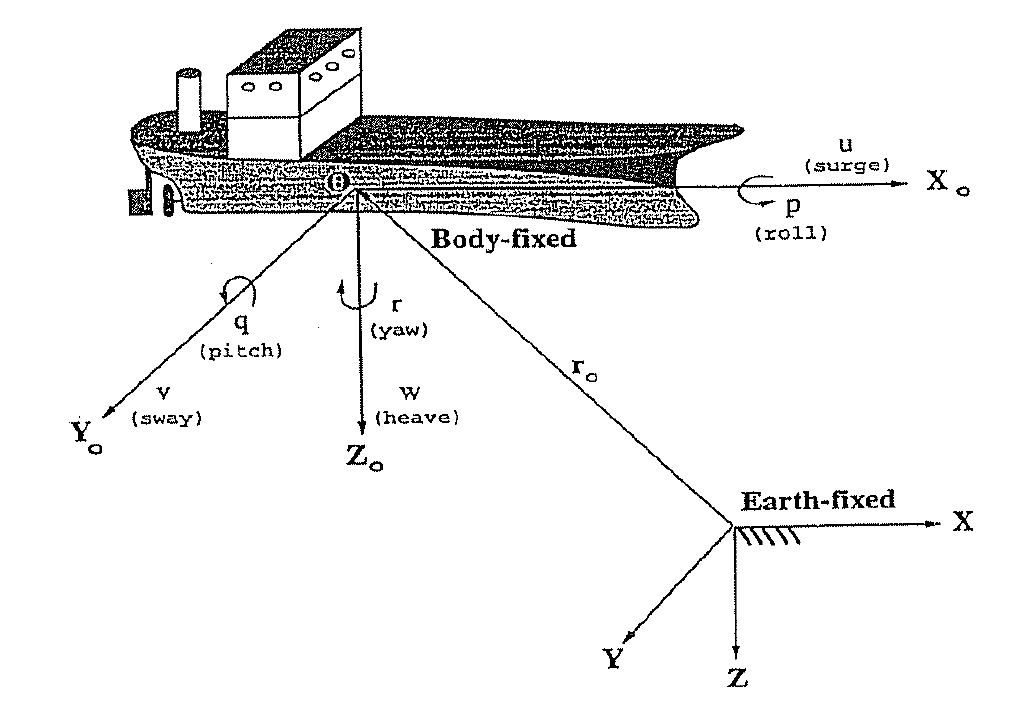
\includegraphics[height = 3.0 in]{/home/rohan/Documents/thesis/coordinate_system.png}}
  \caption{\label{fig-Coordinate System} Body-fixed and earth-fixed reference frames. Figure from \cite{Thor}
}
\end{figure}


The equations described above can be expressed in a more compact form: 
% what is RB
\begin{equation}
\label{eq:motion model AUV}
M_{RB}\mathcal{{V}}^{.}+C_{RB}(\mathcal{V})\mathcal{V}=\tau_{RB}
\end{equation}

Here $\mathcal{V}=[u,v,w,p,q,r]^{T}$ is the body fixed linear and angular velocity and $\tau_{RB}=[X,Y,Z,K,M,N]$ is generalized vector of external forces and moments. $M_{RB}$ is the rigid body inertia matrix and $C_{RB}$ is Coriolis and centripetal matrix. 

The right hand side of the vector \ref{eq:motion model AUV} represents the external forces and moments acting on the vehicle. Fossen \cite{Thor} classifies the forces into 1) Radiation-induced forces 2) Environmental Forces 3) Propulsion Forces

$\tau_{RB}$ can be represented as the sum of these forces.
\begin{equation}
\label{eq:total forces}
 \tau_{RB} = \tau_{H} + \tau_{E} + \tau 
\end{equation}

Here $\tau_{H}$ is the radiation induced forces and moments, $\tau_{E}$ is used to describe the environmental forces and moments and $\tau$ is the propulsion forces and moments. Equations \ref{eq:motion model AUV} and equation \ref{eq:total forces} can be combined to yield the following representation of 6 DOF dynamic equations of motion:
 

\begin{equation}
\label{eq:vehicle hydrodynamics}
M\mathcal{{V}}^{.}+C(\mathcal{V})\mathcal{V}+D(\mathcal{V})\mathcal{V}+g(\eta)=\tau_{E}+\tau%
\end{equation}

where 

$M \triangleq M_{RB} + M_{A}$ ; $C(\mathcal{V}) \triangleq C_{RB}(\mathcal{V} + C_{A}(\mathcal{V})$

$M_A$ is the added inertia  matrix $C_{A}(\mathcal{V})$ is the matrix of hydrodynamic Coriolis and centripetal terms. $g(\eta)$ is the restoring force.

Lammas \cite{Lammas2004} pointed out that navigation equation of an underwater vehicle is-:

\begin{equation}
\label{eq-: navigation equation for AUV}
\mathcal{V}^{.} = M^{-1}(\tau-C(\mathcal{V})\mathcal{V}-D(\mathcal{V})\mathcal{V}-g(\eta))
\end{equation}


$\mathcal{V}^{.}$ can be integrated with time to get velocity.

In the static model the velocity is calculated from a lookup table. In the other model we are computing forces and moments on the fly but the parameters to these forces are considered to be static. The parameters such as density, temperature etc of water can change with time and lead to an inaccurate estimate of velcoity in both the models. Hence the velocity needs to be adapted and Chapter \ref{adapting the motion model} explains how it is done in my algorithm.    


\begin{comment}
The 6-DOF rigid body equations of motions are 

$X=m[u^{.}-vr+wq-x_{G}(q^{2}+r^{2})+y_{G}(pq-r^{.})+z_{G}(pr+q^{.})]$


$Y=m[v^{.}-wp+ur-y_{G}(r^{2}+p^{2})+z_{G}(qr-p^{.})+x_{G}(qp+r^{.})]$

$Z=m[w^{.}-uq+vp-z_{G}(p^{2}+q^{2})+x_{G}(rp-q^{.})+y_{G}(rq+p^{.})]$

$K=I_{x}p^{.}+(I_{z}-I_{y})qr-(r^{.}+pq)I_{xz}+(r^{2}-q^{2})I_{yz}+(pr-q^{.})I_{xy}+m[y_{G}(w^{.}-uq+vp)-Z_{g}(v^{.}-wp+ur)]$

$M=I_{y}q^{.}+(I_{x}-I_{z})rp-(p^{.}+qr)I_{xy}+(p^{2}-r^{2})I_{zx}+(qp-r^{.})I_{yz}+m[y_{G}(u^{.}-vr+wq)-z_{g}(w^{.}-uq+vp)]$

$N=I_{z}r^{.}+(I_{y}-I_{x})pq-(q^{.}+rp)I_{yz}+(q^{2}-p^{2})I_{xy}+(rq-p^{.})I_{zx}+m[x_{G}(v^{.}-wp+ur)-y_{g}(u^{.}-vr+wq)]$

The first three equations represent the translational motion and the
last three represent the rotational motion.$X,Y,Z,K,M,N$ are the
external forces and moments of external forces. $u,v,w$ and $p,q,r$
represent the linear angular velocity of $X,Y,Z$ respectively. $x_{G},y_{G},z_{G}$
represents the center of gravity.

The above equations can be represented in a more compact and vectorial
form.




The forces acting on AUV can be broken down into three classes-:

The external forces and moments vector $\tau_{RB}$is the sum of the
forces listed above 

$\tau_{RB}=\tau_{H}+\tau_{E}+\tau$

Here $\tau_{H}$ is the radiation induced forces and moments, $\tau_{E}$
and $\tau$ are the environmental and propulsion forces and moments respectively. 
A standard numerical ODE integration routine can be used to solve the equation to recover the state.

The input to a motion model is a control command and in our case it is the velocity of the AUV. The velocity is calculated from the propellers. In our algorithm we assume a static model to get a velocity estimate. This can be implemented as a table look-up based on experimental data.
The same control input won't produce the same output every time as it is dependant upon the environment. Therefore we assume a Gaussian distribution over the velocity and try to learn the right parameters over time. 
For my master's thesis we reduce the degrees of freedom and represent the pose of the AUV is two dimensional with orientation. 

In the algorithm the robot can be represented by $X_{t}=(x_{t},y_{t},\theta_{t})$
where $x_{t},y,\theta_{t}$ are the robot's coordinates in x and y
plane and orientation at time $t$. We base our motion model equations on Teddy N. Yap motion model which specifically dealt with odometry to update the pose of the robot. In the set of equations for our model we replace the odometry with velocity. 

$x_{t}=x_{t-1}+V_{t-1}/W_{t-1} \sin(\theta_{t-1})+ V_{t-1}/W_{t-1} \cos(\theta_{t-1} + W_{t-1} \delta t)$

$y_{t}=y_{t-1}+V_{t-1}/W_{t-1} \cos(\theta_{t-1})- V_{t-1}/W_{t-1} \sin(\theta_{t-1} + W_{t-1} \delta t)$

$\theta_{t}=\theta_{t-1}+ W_{t-1} \delta t$


The terms $V_{t}$ and $W_{t}$are the translational and rotational
velocities respectively. They are represented by a Gaussian distribution
to account for the change in forces. They can mathematically represented
as 

$V_{t}\sim\mathcal{{N}}(v_{t},v_{t}^{2}\sigma_{V_{v}}^{2}+w_{t}^{2}\sigma_{V_{w}}^{2}+\sigma_{V_{1}}^{2})$

$W_{t}\sim\mathcal{{N}}(w_{t},v_{t}^{2}\sigma_{w_{v}}^{2}+w_{t}^{2}\sigma_{V_{w}}^{2}+\sigma_{W_{1}}^{2})$

In the above equations $v_{t}$ and $w_{t}$are reported translational
and rotational velocity. $\sigma_{A_{b}}$ describes the contribution
of velocity term b to the variance of the distribution over A. $\sigma_{V_{1}}$and
$\sigma_{W_{1}}$ take into account the independent errors that are
not proportional to translation and rotation of the robot. $\sigma_{V_{v}}^{2}\ensuremath{,}\sigma_{W_{v}}^{2}\ensuremath{,}\sigma_{V_{w}}^{2}\ensuremath{,}\sigma_{W_{w}}^{2}\ensuremath{,}\sigma_{V_{1}}^{2}\ensuremath{,}\sigma_{W_{1}}^{2}$
are the motion parameters that our algorithm intends to learn.
\end{comment}

\section{Particle Filter}
Particle Filter is a state estimation algorithm based on a sampling method for approximating a distribution. Thrun \cite{thrun2005probabilistic} defines particle fitler as an alternative non-parametric implementation of the Bayes filter. It also can be called as a Sequential Monte Carlo(SMC) algorithm. The first attempt to use SMC was seen in simulations of growing polymers by M.N Rosenbluth and A.W. Rosenbluth \cite{rosenbluth1955monte}. Gordon et al. \cite{gordon1993novel} provided the first true implementation of sequential monte carlo algorihtm. 
\begin{comment}
Advantages write  after all introdcution of particle filter

Particle Filters have no restrictions in model i.e. it can be applied to non-Gaussian models,they are super set of other filtering methods i.e. Kalman filter is Rao-Blackwellized particle filter with one particle.Additionally they can model non linear transformations of random variables therefore can be applied to any system and measurement models. All the advantages make them a good alternative to Extended Kalman Filter(EKF) and Unscented Kalman Filter(UKF).
\end{comment}

\begin{figure}
  \centering
     {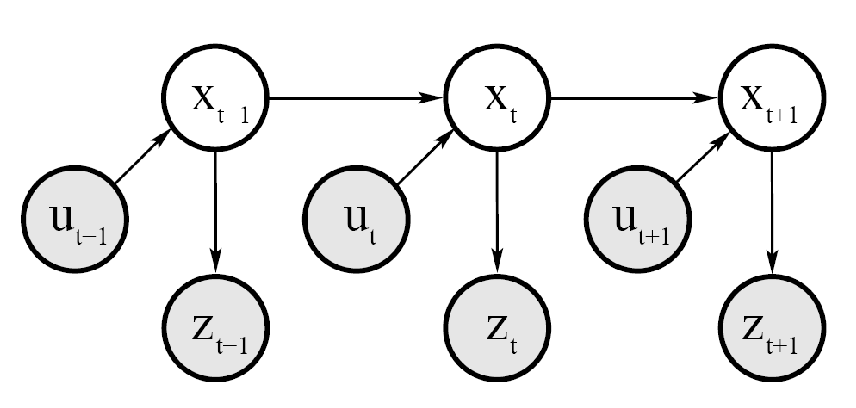
\includegraphics[height = 3.0 in]{../../thesis_work/markov_chain.png}}
  \caption{\label{fig-Markov Chain} A temporal Bayesian model with hidden states $x_{t}$, observations $z_{t}$ and controls $u_{t}$. Figure taken from \cite{thrun2005probabilistic}}
\end{figure}

%\begin{figure}[hbtp]
%\caption{Markov Chain}
%\centering
%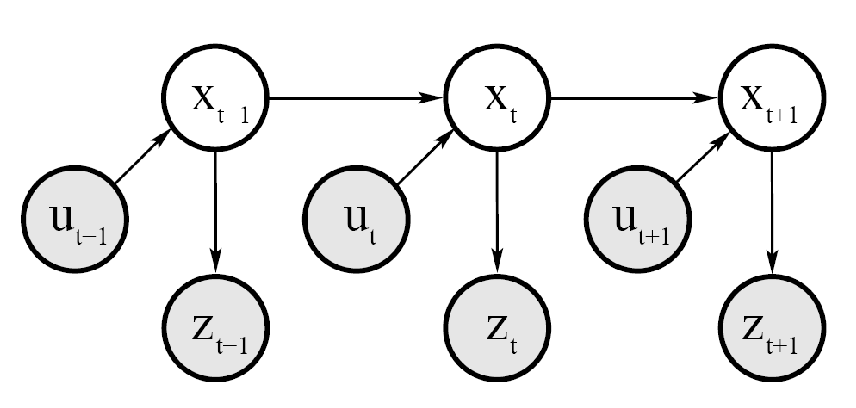
\includegraphics[scale=0.5]{../../thesis_work/markov_chain.png}
%\end{figure}
Thrun \cite{thrun2005probabilistic} stated that the key idea behind particle filter is to represent the posterior bel$(x_{t})$ by a set of random state samples drawn from this posterior. Instead of representing the distribution by a parametric form particle filter represents a distribution by a set of samples drawn from this distribution. In Figure ~\ref{fig: partilce representation} the belief if represented by a set of particles. The representation is a approximation but it is nonparametric and therefore there are advantages of using particle filters as an alternative to Extended Kalman Filter and Unscented Kalman Filter. Particle Filters can represent a broader space of distributions for example non-Gaussian and can model non linear transformations of random variables. In Figure ~\ref{fig: partilce representation} particle filters are shown to model non-linear transformations. 

The objective of particle filters is to estimate the state of the system given the observation variables. They are designed for Hidden Markov Models(Fig ~\ref{fig-Markov Chain}, where the system consists of hidden and observed variables. In this model the state $x_{t}$ is the hidden random variable as it is not directly observed. The state at time $t$ is only dependent upon the state at time $t-1$ and external influences such as control $u_{t}$. The measurement $z_{t}$ depends on the state at time $t$. The knowledge about the influence of the control on the system can be used to calculate a new expected location and the measurement can be combined in a Bayesian way.


\begin{figure}
\centering
{\includegraphics[height = 3.0 in]{/home/rohan/Documents/thesis_work/particle_filter_non_gaussian_thrun.png}}

\caption{\label{fig: partilce representation} The ``particle'' representation used by particle filters. The lower upper right graphs shows samples drawn from a Gaussian random variable, X. These samples are passed through the nonlinear function shown in the upper right graph. The resulting samples are distributed according to the random variable Y. Figure taken from \cite{thrun2005probabilistic}}
\end{figure}

%this figure is copied from Thrun.. How do I reference it???%

The algorithm for particle filters is described below-:

\begin{algorithm}[H]
\label{alg:ParticleFilter}
 \SetAlgoLined
  		 
 \KwIn{$ X _{t-1}$: particle set \\
 $u_{t}$: most recent control \\
 $z_{t}$: most recent measurement}


 \KwOut{ $X_{t}$:particle set }
\Begin{
\For { m=1 to M do} 
{sample $x_{t}^{m}~p(x_{t}|u_{t},x_{t-1}^m)$
$w_{t}^{m}=p(z_{t}|x_{t}^{m})$
$X_{t}^{-}=X_{t}^{-}+(x_{t}^{m},w_{t}^m)$}

\For{m=1 to M do}
{
draw $i$ with probability $\propto$ $w_{t}^{[i]}$
\\
add $x_{t}^{[i]}$ to $X_{t}$}
return $X_{t}$
}
\caption{Particle Filter Algorithm. Algorithm taken from \cite{thrun2005probabilistic}}
\end{algorithm}

In algorithm ~\ref{alg:ParticleFilter} each particle $x_{t}^{m}$ is instantiation of the state at time $t$.  The first step is to generate a hypothetical state $x_{t}^{m}$ for time $t$ based on previous state $x_{t-1}^{m}$ and control $u_{t}$. The particles are samples from the state transition distribution $p(x_{t}|u_{t},x_{t-1})$. The importance factor for each particle $x_{t}^{m}$ is calculated and denoted by $w_{t}^{m}$. Importance factor is defined as the probability of measurement $z_{t}$ under the particle $x_{t}^{m}$. Thus importance factor are used to incorporate the measurements into the particle set. In practice, the number of particles used are a large number(e.g.-:1000).

The key part of the algorithm is the re-sampling step in particle filter algorithm. The algorithm draws M particles with replacement from a temporary particle set $X_{t}^{-}$. The probability of drawing the particles is given by the importance factor. The re-sampling step is a probabilistic implementation of the Darwinian idea of survival of the fittest. It refocuses the particle set to regions in state space with high posterior probability. 

Particle Filters is an integral part of my algorithm to learn the right parameters of the motion model and the way it is used is explained in ~\ref{ch:adapting the motion model}.

\section{Particle smoothing}
\label{ch-: particle smoothing}
The particle filter algorithm as described before is the first step in the Expectation process. The next algorithm that completes the Expectation Step is the particle smoothing. Doucet \cite{doucet2009tutorial} in his paper stated that filtering based on observations received up to the current time is used to estimate the distribution of the current state of an Hidden Markov Model (HMM) whereas smoothing is used to estimate distribution of state at a particular time given all the observations up to some later time (Figure ~\ref{fig:particle smoothing}). Russel and Norving \cite{russell2003artificial} showed that the state of the system is better estimated by smoothing as it incorporates more information than just filtering. We use particle smoothing algorithm proposed by Teddy N Yap and Christian R. Shelton \cite{Yap2008} which was based on the technique presented by Docuet et al. \cite{doucet2000monte} and Godsill et al. \cite{Godsill2004}.
\begin{figure}
\centering
{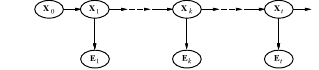
\includegraphics[height = 3.0 in]{/home/rohan/Documents/thesis/smoothing.png}}

\caption{\label{fig: particle smoothing} Smoothing computes $P(X_{k}|e_{1:t})$, the posterior distribution of the state at some past time $k$ given a complete sequence of observations from 1 to $t$. Figure taken from \cite{russell2003artificial}}.
\end{figure}

Particle smoothing is carried out in order to generate samples from the entire joint smoothing density $p(x_{0:T}|u_{1:T},z_{1:T})$. 
The equations described by Yapp \cite{Yap2008} are

\begin{equation}
p(x_{0:T}|u_{1:T},z_{1:T}=\prod_{t=0}^{T}p(x_{t}|x_{t+1:T},u_{1:T},z_{1:T})
\end{equation}

where,

\begin{eqnarray}
p(x_{t}|x_{t+1:T},u_{1:T},z_{1:T}) & = & p(x_{t}|x_{t+1},u_{1:t+1},z_{1:t})\\
 & = & \frac{p(x_{t+1}|x_{t},u_{1:t+1},z_{1:t})p(x_{t}|u_{1:t+1},z_{1:t})}{p(x_{t+1}|u_{1:t+1},z_{1:t})}\\
 & = & \frac{p(x_{t+1}|x_{t},u_{t+1})p(x_{t}|u_{1:t},z_{1:t})}{p(x_{t+1}|u_{1:t+1},z_{1:t})}\\
\label{eq:smoothing_backward} & \alpha & p(x_{t+1}|x_{t},u_{t+1})p(x_{t}|u_{1:t},z_{1:t})
\end{eqnarray}

Equation ~\ref{eq:smoothing_backward} is used to generate states backwards in time give future states. $p(x_{t+1}|x_{t},u_{t+1})$ is the state transition probability and $p(x_{t}|u_{1:t},z_{1:t})$ is obtained by peforming partilce filtering. 
\begin{comment}
 This technique assumes that particle filtering has been carried out on the data set which results in a set of particles $X_{t}$ with their corresponding weights. The states can be generated recursively backwards in time given the future states using equation ~\ref{eq:smoothing_backward}. $p(x_{t}|u_{1:t},z_{1:t})$ can be obtained by performing particle filtering. $p(x_{t}|x_{t+1:T},u_{1:T},z_{1:T}$ can be approximated by particles with modified importance weights $w_{t|t+1}^{[i]} \alpha w_{t}^{[i]}p(x_{t+1}|x_{t}^{[i]},u_{t+1})$ given filtered particles $x_{t}^{[i]}$.  
\end{comment}




Algorithm ~\ref{alg:Particle Smoothing} shows the step involved to sample from the entire joint smoothing density.

\begin{algorithm}[H]
 \SetAlgoLined
  	\label{alg:Particle Smoothing}
 \KwIn{$ X _{t}, t = 0, 1, ..., T$: particle approximations to the posterior pdfs $p (x _{t}|c _{1:t}, s _{1:t}) , t = 0, 1, ..,T$ 
\\
$c _{1:T} = (c _{1}, c _{2}, ..., c _{T} )$: set of controls from time 1 to time T}
 \KwOut{ $x ^{'} _{0:T} = (x ^{'}_{0},x ^{'}_{1}, ...,x^{'}_{T} )$: a sample from the entire joint smoothing density $p (x_{0:T} |c _{1:T} , s _{1:T} )$ }
\Begin{draw \textit{i} with probability $\propto$ $w ^{[i]} _{T}$
$x ^{'} _{T} \leftarrow x^{[i]}_{T}$
\\
\For {$t \leftarrow T-1$ down to 0 do}{\For{ $i \leftarrow 1 to N_{s}$ do}{$w ^{[i]}_{t|t+1} \leftarrow w ^{[i]} _{t}p(x ^{'} _{t+1}|x_{t}^{[i]},u _{t+1})$}draw \textit{i} with probability $\propto w ^{[i]} _{t|t+1}$\\ $x^{'} \leftarrow x^{[i]}_{t}$}}
	\caption{Sample the entire joint smoothing density $p(x_{0:T}|c_{1:T},s_{1:T})$}
	
\end{algorithm}

In the first step of the algorithm a particle is drawn with probability proportional to the filtered weight of the particles. The next step is to move a time step back and modify the weights of the particles by calculating the new smoothed weights. The new smoothed weights are the product of state transition probability $p(x ^{'} _{t+1}|x_{t}^{[i]},u _{t+1})$ and the weight of the particle $w_{t}^{[i]}$. The next step in the algorithm is to draw particles with probability proportional to new smoothed weights $w_{t|t+1}^{[i]}$.  The sequence of particles $x^{'}$ drawn from joint smoothing density $p(x_{0:T}|c_{1:T},s_{1:T})$ from time 0 to time T form a sampled trajectory $x^{'}_{0:T} \triangleq (x^{'}_0,x^{'}_1,.....,x^{'}_T)$.
 
 
 





\chapter{Learning the motion model}
\label{learning the motion model}
\section{Introduction}
\subsection{Work done so far on learning motion model}
The process of calibration has been discussed right from when robotics was introduced and the literature is full of different methods to calibrate a robot (eg-: \cite{cox1990autonomous} \cite{vukobratovic1989introduction}). Virtually all the methods discussed before Roy's work \cite{Roy} required human intervention and assumed the world to be static. These methods required a human to have experience and a device to measure the exact movement of a robot to calibrate. The most important assumption that these methods made was that the physics of a robot never changed and operated in a static environment. 

Roy and Thrun first proposed an online self-calibration method \cite{Roy} in 1999 that adapted to changes that occurred during the lifetime of a robot. The algorithm was designed for land robots where the final pose was given by equations described below

\begin{equation}
x^{'}=x+Dcos(\theta+T)
y^{'}=y+Dsin(\theta+T)
\theta^{'}=(\theta+T)mod2\pi
\end{equation}

$D$ and $T$ are the true translational and rotation of a robot. The measured translational and rotational is $d$ and $t$ and if robot's odometry is accurate then $D=d$ and $T=t$. In practice there is a difference and Roy represents $D$ and $T$ by equations ~\ref{eq-: thrun_noise_D} and ~\ref{eq-: thrun_noise_T} respectively.

\begin{equation}
\label{eq-: thrun_noise_D}
D= d+ \sigma_{trans}d+\epsilon_trans
\end{equation}

\begin{equation}
\label{eq-: thrun_noise_T}
  T= t+ \sigma_{rot}d+\epsilon_{rot}
\end{equation}

$\epsilon_trans$ and $\epsilon_{rot}$ are the random variables with zero mean. $\sigma_{trans}$ and $\sigma_{rot}$ are the systematic error, drift.  The algorithm they propose is used to estimate $\sigma_{trans}$ and $\sigma_{rot}$ using sensor data collected throughout robot's motion. They treat the problem as maximum likelihood estimation problem where the parameters are estimated under a dataset $z$ (equations ~\ref{eq-:max_likelihood_thrun}) .

\begin{equation}
\label{eq-:max_likelihood_thrun}
 (\sigma_{trans}^{*},\sigma_{rot}^{*}) = argmax P(\sigma_{trans},\sigma_{rot}|z)
\end{equation}

Austin and Eliazar \cite{Eliazar2004} proposed a different method to achieve the same goals proposed by Roy and Thrun. Their algorithm was different from Roy and Thrun for two reasons. Firstly, Austin ad Eliazar used a more general model which incorporated independence of motion terms. Secondly, the method was able to estimate parameters for non systematic errors as well. 
The motion model proposed by them to account is described below.
\begin{equation}
	\begin{aligned}
	x^{'}&=&x+Dcos(\theta+T/2) \\
	y^{'}&=&y+Dsin(\theta+T/2) \\
	\theta^{'}&=&(\theta+T/2)mod2\pi
	\end{aligned}
\end{equation}
As the turn and drive commands are performed independently therefore to not violate this assumption this model makes T reasonably small and it is absorbed as part of noise. To estimate non-systematic errors the true translational($D$ and rotation($T$) are represented by normal distribution with mean $d$ and $t$ and the variance will scale with $d^2$ and $t^2$ as shown in equation ~\ref{eq-:noise_model_eliazar}
\begin{equation}
\label{eq-:noise_model_eliazar}
\begin{aligned}
D &\sim& \mathcal{{N}}(d\mu_{D_{d}}+t\mu_{D_{t}},d^2\sigma_{D_{d}}^2+t^2\sigma_{D_{t}}^2)\\
T &\sim& \mathcal{{N}}(d\mu_{T_{d}}+t\mu_{T_{t}},d^2\sigma_{T_{d}}^2+t^2\sigma_{T_{t}}^2)
\end{aligned}
\end{equation}

where $\mu_{A_{b}}$ is the coefficient for the contribution of odometry term b to the mean of the distribution over A. The algorithm is used to learn these set of mean and variances.

The method by Austin an Eliazar used Expectation Maximization framework to learn the parameters of the motion model for land robots. In the E step particle filtering and smoothing were performed to get a set of trajectories. In M step the maximum likelihood values of parameters given the trajectories was calculated. Teddy Yapp \cite{Yap2008} used the same framework and learned parameters for motion as well as sensor model of land robots (Figure ). They adopted the same motion model by with slight different noise model as shown in equation ~\ref{eq-:noise_model_yapp}.
\begin{figure}
  \centering
     {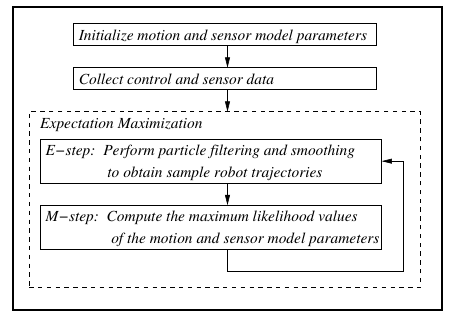
\includegraphics[height = 3.0 in]{/home/rohan/Documents/thesis_work/parameter_estimation_yapp.png}}
  \caption{\label{fig-parameter_estimation Yapp} Block Diagram for the parameter estimation framework. Figure taken from \cite{Yapp2008}.}
\end{figure}

\begin{equation}
\label{eq-:noise_model_yapp}
\begin{aligned}
D &\sim& \mathcal{{N}}(d,d^2\sigma_{D_{d}}^2+t^2\sigma_{D_{t}}^2+\sigma_{D_{1}}^2) \\
T &\sim& \mathcal{{N}}(t,sigma_{T_{d}}^2+t^2\sigma_{T_{t}}^2+\sigma_{T-{1}}^2)
\end{aligned}
\end{equation}

The extra constant terms $\sigma_{D_{1}}$ and $\sigma_{T_{1}}$ are added to account for the errors that are not proportional to the translation or rotation of a robot. 

All the work above was done to calibrate our models and Hegrenaes \cite{Hegrenæs2008} in his work showed the importance of motion model for navigation in underwater vehicle. The proposed an novel approach for navigation systems in which knowledge about the vehicle dynamics was used to aid the Inertial Navigation System(INS). The new navigation system was tested on real dataset collected by an AUV.

For navigation in AUV velocity of the vehicle needs to be estimated and sensors such as IMU, DVL etc. are used. In a traditional INS system the key component is an IMU and a set of navigation equations. The reading from accelerometer and gyroscope are integrated to get an estimate of velocity, position and orientation. The reading from such sensors consist of inherent errors and leads to drift in the INS system. Generally sensors such as surface GPS, DVL etc. are an aiding system to the INS (Figure ~\ref{fig-INS systems(a)} ). Combination of such as system leads to better estimate of velocity, position and orientation \cite{leonard1998autonomous}. 

Hergreanaes points out an alternative velocity information such as velocity estimate through vehicle dynamics is required because there are situations where it is not possible for the AUV to surface and get a GPS reading or DVL measurement needs to be discarded due to poor quality. The high level system outline for such a model is shown in Figure ~\ref{fig-INS systems}(b).

The system is very similar to traditional INS except that the vehicle model output in also integrated to the system. The vehcile model output doesn't require any extra instruments therefore can be easily applied to any vehicle. An alternative velocity estimate aids the INS where DVL readings are lacking as well as gives redundancy to the system. 




\begin{figure}
  \centering
  \subfigure[Traditional aided INS]{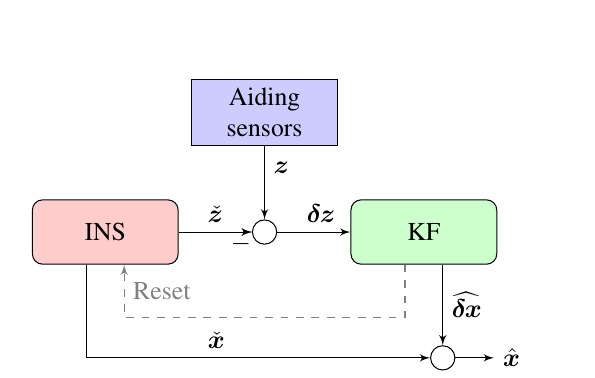
\includegraphics[width = 2.75 in]{/home/rohan/Documents/thesis_work/model_aided_intertial_nvaigation_system_traditional.png}}\qquad
  \subfigure[Mode-aided INS]{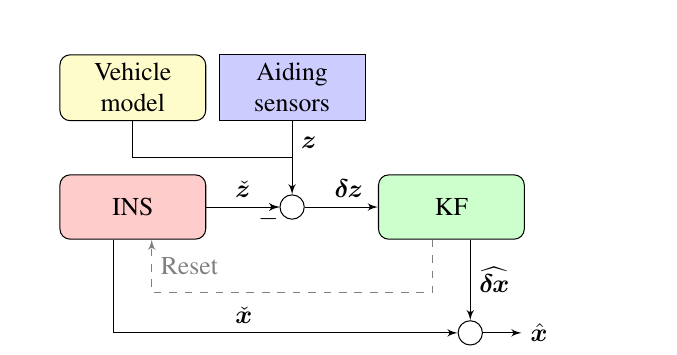
\includegraphics[width = 2.75 in]{/home/rohan/Documents/thesis_work/model_aided_intertial_nvaigation_system_model.png}}
 
  \caption{\label{fig-INS systems}High level system outline. The vehicle model can be used in parallel to external aiding sensors. Figure taken from \cite{Hegrenæs2008}}
\end{figure}

All the above calibration methods are designed for odometric based motion models and for land robots. The use of vehicle model to aid the INS for navigation purposes shows us the importance of an adaptive motion model. The algorithm that I propose is for underwater vehicles and velocity based motion model. The process to adapt the motion model is similar to the previous work by Yapp and Eliazar and our approach is described in rest of the chapters.

\subsection{General Architecture}
In this section we give an overview of the system and point out the differences in my system(Figure ~\ref{fig:general archi}) as compared to the existing system proposed by Yapp \cite{Yap2008}. 
\begin{figure}
  \centering
     {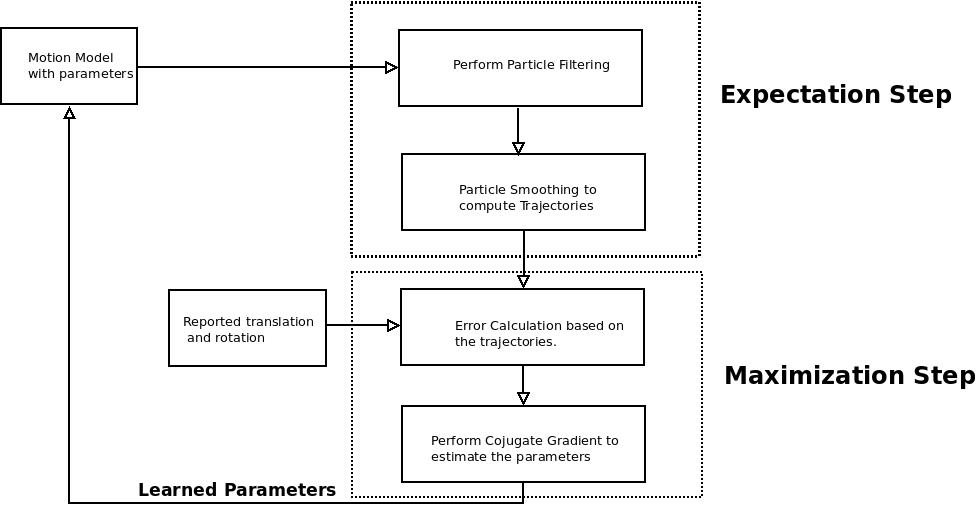
\includegraphics[height = 3.0 in]{Diagram1.jpeg}}
  \caption{\label{fig-General Architecture} Block diagram for adapting motion model.}
\end{figure}
Figure ~\ref{fig- General Architecture} is an outline of the proposed system. The motion and sensor models are initialized with a set of parameters. Given the motion model $p(x_{t}|x_{t-1},u_{t})$, sensor model $p(z_{t}|x_{t})$ and the pose $p(x_{t-1})$ of a robot we can perform particle filtering using Algorithm ~\ref{alg:ParticleFilter}. It is performed to estimate the pose $p(x_{t})$ of a robot at next time step. 

The key ingredient to learn the motion model is to have an estimate of ground truth. To get an idea of ground truth particle smoothing (algorithm ~\ref{alg:Particle Smoothing}) is performed on the particle set produced by particle filtering. The algorithm can be repeated several times to get a set of trajectories. Particle filtering and smoothing are the key algorithm for the Expectation Step. 

The reported translational and rotational movement of a robot is recorded for every time step. Based on the trajectories and reported movements the errors are calculated at each time step. After we have a set of errors we perform Newton Conjugate gradient on the error function to estimate the set of parameters. This completes the Maximization Step.

The learned parameters are reassigned to the motion model and helps in adapting our model to changes in robot and the environment. The whole algorithm is repeated at every time step so that we can dynamically learn the right parameters.

The system proposed for parameter estimation is similar to the system by Yapp \cite{Yap2008}. I use the same EM framework and conjugate gradient to learn the right parameters for the model. The difference lies that the motion model learned is a velocity based motion model as compared to odometry based model. Secondly we focus on underwater environments and therefore use side sonar images to calculate landmarks on the fly for our sensor model as compared to a static map.

\section{Adapting Motion Model}
\subsection{Expectation Maximization}

Expectation Maximization is an iterative process of finding maximum likelihood of parameters of a model which depend upon hidden variables. It is used to estimate unknown parameters $\theta$ given the observed data $X$. A complete dataset can be represented by ${X,Z}$ where $Z$ is a non-observed (hidden, latent) variable. In practice a complete dataset is not given and only a set of observations or incomplete dataset $X$ is found. The hidden variables are important to a problem but complicate the learning process ~\cite{russell2003artificial}. In order to learn with hidden variables Dempster et al. \cite{dempster1977maximum} proposed a method to maximize the probability of the parameters $\theta$ give the dataset $X$ with hidden variables $Z$ called as EM.

\begin{equation}
\label{eq-:em_description}
\theta^{*}=arg max_{\theta} \int p(\theta,Z|X)dZ
\end{equation}

The key idea behind the EM algorithm is to alternate between estimating parameters $\theta$ and hidden variable $Z$.
The E step consists of finding the posterior distribution of hidden variables $p(Z|X,\theta^{old})$ given the current estimate of parameters $\theta^{old}$. The posterior distribution it used to find a expectation of the likelihood of the data for some parameter $\theta$ as shown in equation ~\ref{eq-: maximization}. 
\begin{equation}
\label{eq-:maximization}
\mathcal{Q}(\theta,\theta^{old})=\sum_{Z}p(Z,X|\theta^{old}) \ln p(X,Z|\theta)
\end{equation}
In the M step we maximize the function as shown in  to estimate the new parameters $\theta^{new}$.
\begin{equation}
\theta^{new}=arg max_{theta} \mathcal{Q}(\theta,theta^{old})
\end{equation}

The objective as described by Minka \cite{minka1998expectation} is to maximize $\mathcal{Q}(\theta,\theta^{old})$ and we want an updated estimate of $\theta^{new}$ such that 
\begin{equation}
\theta^{new}>\theta^{old}
\end{equation}
or we want to maximize the difference,
\begin{equation}
\mathcal{Q}(\theta^{new})-\mathcal{Q}(\theta^{old})=\ln P(X|\theta^{new}) - \ln P(X|\theta^{old})
\end{equation}
The above equations with hidden variables can be written as
\begin{equation}
\label{eq-:derivation_em}
\mathcal{Q}(\theta^{new})-\mathcal{Q}(\theta^{old})=\ln(\sum P(X|z,\theta^{new}) P(Z|\theta^{new})) - \ln P(X|\theta^{old})
\end{equation}

Using Jensen's Equality it can be show that,
\begin{equation}
\ln \sum_{i=1}^{n}\lambda_{i}x_{i} \geq \sum_{i=1}^{n}\lambda_{i}\ln(x_{i})
\end{equation}
for constants $\lambda_{i} \geq 0$ with $\sum_{i=1}^{n}\lambda_{i}=1$. This can be applied to equation ~\ref{eq-: derivation_em} and $\lambda=P(Z|X,\theta^{old})$. As $P(Z|X,\theta^{old})$ is a probability measure we have $P(Z|X,\theta^{old}) \geq 0$ and $\sum_{Z}P(Z|X,\theta^{old})=1$.

\begin{eqnarray}
Q(\theta^{new})-Q(\theta^{old}) & = & \ln(\sum_{Z}P(X|Z,\theta^{new})P(Z|\theta))-\ln P(X|\theta^{old})\\
 & = & \ln(\sum_{Z}P(X|Z,\theta^{new})P(Z|\theta).\frac{P(Z|X,\theta^{old})}{P(Z|X,\theta^{old})})-\ln P(X|\theta^{old})\\
 & = & \ln(\sum_{Z}P(z|X,\theta^{old})\frac{P(X|Z,\theta^{new})P(Z|\theta^{new}}{P(Z|X,\theta^{old})})-\ln P(X|\theta^{new})\\
 & \geq & \sum_{Z}P(Z|X,\theta^{old})\ln(\frac{P(X|Z,\theta^{new})P(Z|\theta^{new})}{P(Z|X,\theta^{old})})-\ln P(X|\theta^{old})\\
 & = & \sum_{Z}P(Z|X,\theta^{old})\ln(\frac{P(X|Z,\theta^{new})P(Z|\theta^{new})}{P(Z|X,\theta^{old})P(X|\theta^{old})})\\
 & \triangleq & \triangle(\theta^{new}|\theta^{old})
\end{eqnarray}
We continue by writing

$\mathcal{Q}(\theta^{new})\geq\mathcal{Q}(\theta^{old})+\triangle(\theta^{new}|\theta^{old})$

and for convenience define,

$q(\theta^{new}|\theta^{old})\triangleq\mathcal{Q}(\theta^{old})+\triangle(\theta^{new}|\theta^{old})$

The function $q(\theta^{new}|\theta^{old})$ is bounded by the likelihood
functions $\mathcal{Q}(\theta^{new})$. We need to choose values of
$\theta^{new}$so that $\mathcal{Q}(\theta^{new})$ is maximized.
The new updated value is denoted by $\theta_{n+1}.$
\begin{eqnarray}
\theta_{n+1} & = & argmax_{\theta}\{q(\theta^{new}|\theta^{old})\}\\
 & = & argmax_{\theta}\{\mathcal{Q}(\theta^{old})+\sum_{Z}P(Z|X,\theta^{old})\ln(\frac{P(X|Z,\theta^{new})P(Z|\theta^{new})}{P(Z|X,\theta^{old})P(X|\theta^{old})})\\
 & = & argmax_{\theta}\{\sum_{Z}P(Z|X,\theta^{old})\ln(P(X|Z,\theta^{new})P(Z|\theta^{new})\}\\
 & = & argmax_{\theta}\{\sum_{Z}P(Z|X,\theta^{old})\ln P(X,Z|\theta^{new})\}\\
\end{eqnarray}

We use the EM algorithm as described by Christopher M. Bishop in his book \cite{bishop2006pattern}. The steps taken in EM algorithm are described below -:
\\
1. Have an initial estimate of the parameters $\theta ^{old}$
\\
2. \textbf{E Step:} Evaluate $p(Z|X,\theta^{old})$
\\
3. \textbf{M Step:} Evaluate $\theta ^{new} = arg max _{\theta} L(\theta,\theta^{old})$
\\
\hspace*{20 mm} where 
$L(\theta,\theta^{old})=\Sigma _{Z} p(Z|X,\theta_{old}) \log p(X,Z|\theta)$
\\
4. Check for the convergence of either the log likelihood or the parameter values. If the convergence criterion is not satisfied then let
\\
\hspace*{20 mm} $\theta \leftarrow \theta^{new} $
\\
and return to step 2
\\
There are various convergence techniques that can be applied in step 4. In our algorithm we use Newton Conjugate Gradient to estimate the right parameters. It is important to point that EM algorithm is local optimization technique and there are situations where it can get stuck in local optimum. 		


\subsection{Parameter Estimation}
\label{ch:adapting the motion model}
In this section we give a detailed explanation of the method proposed to learn motion model. As stated in Chapter ~\ref{chap-:Motion Model} to calculate the position of AUV we need to estimate velocity and feed it to the navigation equation ~\ref{eq-: navigation equation for AUV}. As we are operating in a dynamic environment there are various factors that can lead to changes in our motion model. To adapt the motion model we represent the velocity as a Gaussian distribution. We assume the distribution to be Gaussian as sum of several random noises leads to a such a distribution.   The algorithm described here is used to estimate parameters of the distribution. Another assumption for the algorithm that we represent the pose of an AUV in two dimension as compared to six. 

The velocity based motion model equations used in the algorithm are 

\begin{equation}
 x_{t}=x_{t-1}+V_{t-1}/W_{t-1} \sin(\theta_{t-1})+ V_{t-1}/W_{t-1} \cos(\theta_{t-1} + W_{t-1} \delta t)
\end{equation}

\begin{equation}
\label{eq:velocity motion model_y}
y_{t}=y_{t-1}+V_{t-1}/W_{t-1} \cos(\theta_{t-1})- V_{t-1}/W_{t-1} \sin(\theta_{t-1} + W_{t-1} \delta t)
\end{equation}

\begin{equation}
\label{eq:velocity motion model_theta}
\theta_{t}=\theta_{t-1}+ W_{t-1} \delta t
\end{equation}

where,
\begin{equation}
V \sim \mathcal{N}(v_{t},v_{t}^{2}\sigma_{V_{v}}^{2}+w_{t}^{2}\sigma_{V_{w}}^{2}+\sigma_{V_{1}}^{2})
W \sim \mathcal{N}(w_{t},v_{t}^{2}\sigma_{W_{v}}^{2}+w_{t}^{2}\sigma_{W_{w}}^{2}+\sigma_{W_{1}}^{2})
\end{equation}


The translational and rotational velocity are represented by a Gaussian distribution with mean as reported translational $v$ and rotational $t$ velocity respectively. $\sigma_{A_{b}}$ represents the contribution of the velocity term b to the variance of the distribution over A. $\sigma_{V_{1}} $ and $\sigma_{w_{1}}$ are added to the motion model to account for errors that are not directly proportional to the translation and rotation of a robot.

Putting the whole problem of estimating parameters in EM framework, we define the parameters of the motion model that we want to learn are
$\theta={\sigma_{V_{v}}^{2},\sigma_{V_{w}}^{2},\sigma_{V_{1}}^{2},\sigma_{W_{v}}^{2},\sigma_{W_{t}}^{2},\sigma_{W_{1}}^{2}}$
The data Z from which the parameters can be learnt are
 
$Z={u_{1:T},z_{1:T}}$
where,
$u_{1:T}$ and $z_{1:T}$ are the history of control and sensor readings.

The robot's trajectory is the hidden variable in the system as it not directly observable. 
$r=x_{0:T}$

The first step in an EM algorithm is to initialize the set of parameters $\theta$ with some initial values. In the E step we calculate the expectation of $\log p(r,Z|\theta)$ with respect to distribution $p(r|Z,\theta)$. The distribution can be also be represented by the entire join smoothing density $p(x_{0:T}|u_{1:T},z_{1:T})$. To approximate the E step joint smoothing density particle filtering and smoothing is performed to calculate a set of robot trajectories as discussed in section ~\ref{ch-: particle smoothing}. In the M step we treat the set of trajectories as ground truth as use them to compute the maximum likelihood of parameters. The algorithm keeps on alternating between the E and M step until convergence. 

For calculating the maximum likelihood values for parameters we need to calculate the motion errors $epsilon_{T_{t}},epsilon_{D_{t}}$ based on robot trajectory and the contribution of translational $v$ and rotational $t$ velocity to the errors.

\begin{eqnarray}
\epsilon_{T_{t}}^{[j]}&=&(\theta_{t_{+1}}^{'[j]}-\theta_{t}^{'[j]}-r_{t}^{''})mod2\pi\\
\epsilon_{D_{t}}^{[j]}&=&(x_{t+1}^{'[j]}-x_{t}^{'[j]})cos(\theta_{t}^{'[j]}+\frac{r_{t}^{''}+\epsilon_{T_{t}}^{[j]}}{2}+(y_{t+1}^{'[j]}-y_{t}^{'[j]})sin(\theta_{t}^{'[j]}+\frac{r_{t}^{''}+\epsilon_{T_{t}}^{[j]}}{2})-d_{t}^{''}
\end{eqnarray}

The distribution that represents these errors are 
\begin{eqnarray}
\epsilon_{V_{t}}^{[j]}&\sim&\mathcal{{N}}(0,v_{t}^{2}\sigma_{V_{v}}^{2}+w_{t}^{2}\sigma_{V_{w}}^{2}+\sigma_{V_{1}}^{2})\\
\epsilon_{W_{t}}^{[j]}&\sim&\mathcal{{N}}(0,v_{t}^{2}\sigma_{w_{v}}^{2}+w_{t}^{2}\sigma_{V_{w}}^{2}+\sigma_{W_{1}}^{2})
\end{eqnarray}

where j stands for sampled trajectory.

The likelihood functions are 
\begin{eqnarray}
\mathcal{Q}_{\epsilon_{D}}(\sigma_{V_{v}}^{2},\sigma_{V_{r}}^{2},\sigma_{V_{1}}^{2}) & = & p(\{\epsilon_{V_{v}}^{[j]}\}|u_{1:T},\{k_{0:T}^{[j]}\})\\
 & = & \prod_{j}\prod_{t=0}^{T-1}\frac{1}{\sqrt{2\pi(v_{t}^{2}\sigma_{V_{v}}^{2}+r_{t}^{2}\sigma_{V_{r}}^{2}+\sigma_{V_{1}}^{2})}}*\exp(\frac{(\epsilon_{V_{t}}^{[j]})^{2}}{2(d_{t}^{2}\sigma_{V_{v}}^{2}+r_{t}^{2}\sigma_{V_{r}}^{2}+\sigma_{V_{1}}^{2})}
\end{eqnarray}



\begin{eqnarray*}
\mathcal{Q}_{\epsilon_{T}}(\sigma_{W_{d}}^{2},\sigma_{W_{r}}^{2},\sigma_{W_{1}}^{2}) & = & p(\{\epsilon_{W_{t}}^{[j]}\}|u_{1:T},\{k_{0:T}^{[j]}\})\\
 & = & \prod_{j}\prod_{t=0}^{T-1}\frac{1}{\sqrt{2\pi(v_{t}^{2}\sigma_{W_{d}}^{2}+r_{t}^{2}\sigma_{W_{r}}^{2}+\sigma_{W_{1}}^{2})}}*\exp(\frac{(\epsilon_{W_{t}}^{[j]})^{2}}{2(v_{t}^{2}\sigma_{W_{d}}^{2}+r_{t}^{2}\sigma_{W_{r}}^{2}+\sigma_{W_{1}}^{2})})
\end{eqnarray*}


The estimate the parameters we get the maximum likelihood estimates 

\begin{eqnarray}
\sigma_{V_{v}}^{2*},\sigma_{V_{r}}^{2*},\sigma_{V_{1}}^{2*} & = & argmax_{\sigma_{V_{v}}^{2},\sigma_{V_{r}}^{2},\sigma_{V_{1}}^{2}}\mathcal{Q}(\sigma_{V_{v}}^{2},\sigma_{V_{r}}^{2},\sigma_{V_{1}}^{2})\\
\sigma_{W_{d}}^{2*},\sigma_{W_{r}}^{2*},\sigma_{W_{1}}^{2*} & = & argmax_{\sigma_{W_{d}}^{2},\sigma_{W_{r}}^{2},\sigma_{W_{1}}^{2}}\mathcal{Q}(\sigma_{W_{d}}^{2},\sigma_{W_{r}}^{2},\sigma_{W_{1}}^{2})
\end{eqnarray}

We maximize the log likelihood function via Newton conjugate gradient method with respect to motion model parameters. Conjugate gradient is a method to determine the minimum or maximum of a function \cite{shewchuk1994introduction}. Generally it requires the gradient of the function. In this method the gradient of the function is taken as the first search direction while the next search direction are chosen in such a way that they are orthogonal to all previous search directions. The gradient of log likelihood functions are 

\begin{eqnarray}
\mathcal{{L}}(\sigma_{V_{v}}^{2},\sigma_{V_{w}}^{2},\sigma_{V_{1}}^{2})&=&-\frac{1}{2}\sum_{j}\sum_{t=0}^{T-1}[\log2\pi+\log(v_{t}^{2}\sigma_{V_{v}}^{2}+w_{t}^{2}\sigma_{V_{w}}^{2}+\sigma_{V_{1}}^{2})+\frac{(\epsilon_{V_{t}}^{[j]})^{2}}{v_{t}^{2}\sigma_{V_{v}}^{2}+w_{t}^{2}\sigma_{V_{r}}^{2}+\sigma_{V_{1}}^{2}}\\
\mathcal{{L}}(\sigma_{W_{v}}^{2},\sigma_{W_{w}}^{2},\sigma_{W_{1}}^{2})&=&-\frac{1}{2}\sum_{j}\sum_{t=0}^{T-1}[\log2\pi+\log(v_{t}^{2}\sigma_{W_{v}}^{2}+w_{t}^{2}\sigma_{W_{w}}^{2}+\sigma_{W_{1}}^{2})+\frac{(\epsilon_{W_{t}}^{[j]})^{2}}{v_{t}^{''2}\sigma_{W_{v}}^{2}+w_{t}^{''2}\sigma_{W_{w}}^{2}+\sigma_{W_{1}}^{2}}
\end{eqnarray}
 



\begin{comment}
\section{Application}
In this chapter we describe a specific application for learned motion model in underwater vehicles. A typical navigation sensor system would consists of Inertial Navigation Systems(INS) and some standard compass and pressure sensor. In some of the systems we could have position updates from long baseline(LBL),ultra short baseline(USBL) acoustics and surface GPS. Some high end systems would have Doppler Velocity Log(DVL) which estimates speed over ground or water. These systems are sometimes incorporated to limit the drift of Inertial Navigation System[refer the paper]. Even when a DVL is included there are situations in which DVL fails or the reading have to be discarded due to poor quality. 

We need some sort of alternative velocity information that doesn't depend upon external sensors in order to compensate for the drift in INS. To get an estimate of velocity we can use the kinetic vehicle model to aid the INS. 
\begin{figure}[hbtp]
\caption{Traditional aided INS}
\centering
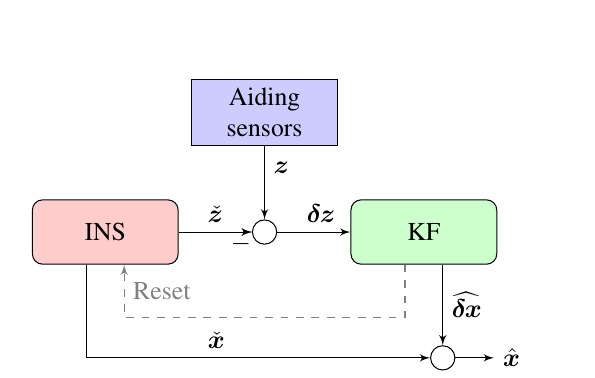
\includegraphics[scale=1.0]{/home/rohan/Documents/thesis_work/model_aided_intertial_nvaigation_system_traditional.png}
\end{figure}

\begin{figure}[hbtp]
\caption{Traditional aided INS}
\centering
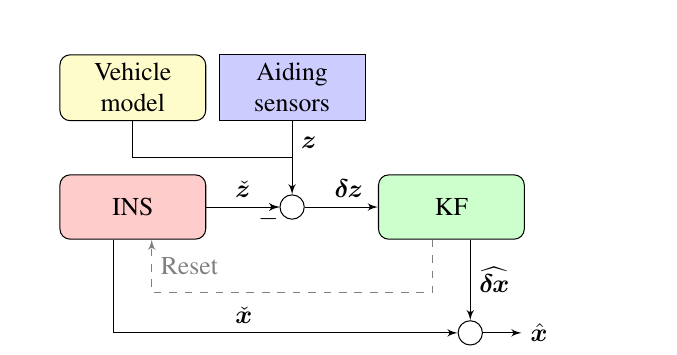
\includegraphics[scale=1.0]{/home/rohan/Documents/thesis_work/model_aided_intertial_nvaigation_system_model.png}
\end{figure}
In the traditional aided INS the readings from gyro and accelerometer measurements from the IMU are integrated over time to give an estimate of velocity,position and orientation. Due to the inherent errors in the gyros and accelerometers there is a drift in  the INS system. There are aiding sensors such as DVL and surface GPS to compensate the drift for the IMU. The reading from the sensors are fused using a Bayes filters to get an enchained estimate of velocity ,position and orientation. 

In the model aided INS the IMU suffers from the same drift but the output from the model is treated analogously to that of an external aiding sensor. In this system the DVL in traditional INS systems are replaced by vehicle model. The output from the model i.e. the velocity estimate is fused with the readings from the INS by a Bayes filter. The integrating of vehicle model with the IMU systems help in systems which lack external velocity measurements. The other implication is in systems where redundancy and integrity is important e.g. during sensor drop outs or sensor failures.

This specific application shows the importance of having a accurate motion model. As stated in earlier chapters the motion model can change due to various factors and would have a direct impact on the navigation systems of underwater vehicles.Wrong estimates from the motion model will not benefit INS systems and overall lead to wrong estimate about the position and orientation of the vehicle. Our algorithm shows on how to learn the motion model on the fly which can lead to better estimate of the velocity and therefore accurate navigation systems.

As you can see in the figure the input to the motion model is a control command and output is the velocity estimate. In HUGIN 4500 they had implemented a static motion model as table look up based on experimental data i.e.
$u_{r}=f(n_{s})$  where $n_{s}$ is the control system set point. The velocity estimate $u_{r}$ is fused with the reading from IMU to get a better estimate of the position of the AUV. As shown before we try to learn the motion model to find the best estimate for the velocity so that it can aid the INS in this particular application. 
\end{comment}
\chapter{Results and Experimental Setup}
In this chapter we describe the experimental setup of the simulator to test our algorithm. To demonstrate the effectiveness of our approach the results from the simulated experiment are also shown.
\section{Experimental Setup}
To test our algorithm for learning the motion model we create a simulated world(Figure ~\ref{fig-: simulation world}). The world size of our simulation is 400X400 with four landmarks shown in blue dots. The red * shows the location of the robot and blue triangle is the location estimate of the  robot by particle filters. The robot is moving with a constant forward and rotational velocity throughout the experiment. In simulation the robot can measure its distance from all four landmarks at all time. The sensor noise in the simulation can be varied in between the experiment. The particle size is 500 and is constant throughout the experiment. Table ~\ref{tab- constant parameters} shows the summary of variables for the experiment to test the effectiveness of our algorithm to learn a motion model.
\begin{table}[tbh]
\centering
\begin{tabular}{|r|r|}
    \hline
    & Experiment \\
    \hline \hline
    World Size & 400 units X 400 units\\
    \hline
    Total timesteps & 400  \\
    \hline
    No. of sensor readings & 400 \\
    \hline
    Translational Velocity & 3 units/timestep \\
    \hline
    Rotational Velocity & 01. units/timestep \\
    \hline
\end{tabular}
 \caption{\label{tab-constant paramters}Summary of adapting motion model experiment.}
\end{table}

\begin{figure}
  \centering
     {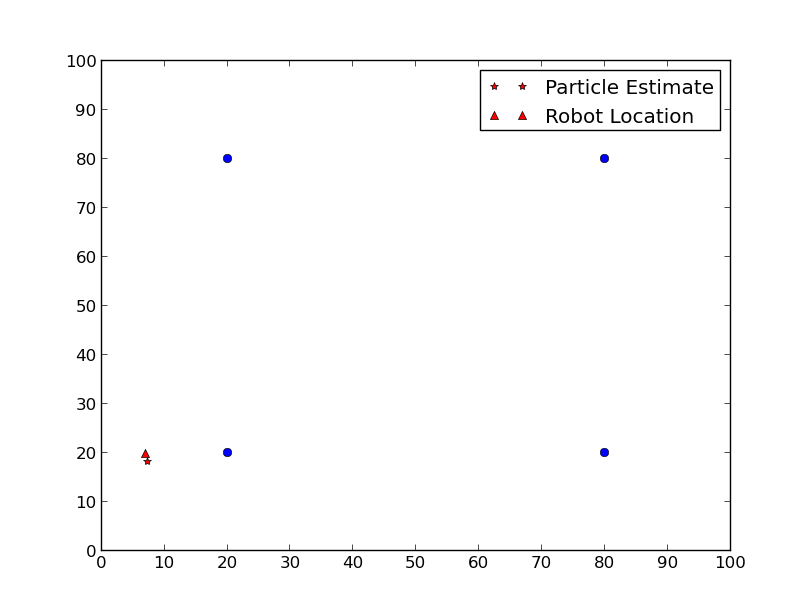
\includegraphics[height = 3.0 in]{0.png}}
  \caption{\label{fig-: simulation world}The simulation environment consisting of the robot(triangle) and the particle estimate of teh location(star). The blue dots represent the landmarks.}
\end{figure}


At the start of the experiment  the initial location of the robot and particle filters are randomly initialized (Figure ~\ref{fig-: movement simulation world} (a)). The robot is moved by a constant velocity and Figure ~\ref{fig-: movement simulation world (b)(c)(d)} shows the updated location of the robot as well as an estimate by particle filters of the robot's location.



\begin{figure}
  \centering
  \subfigure[]{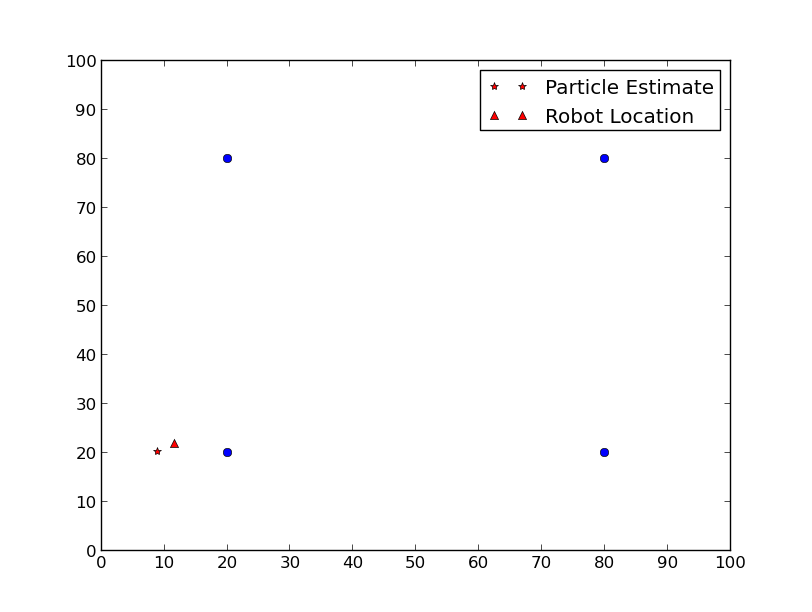
\includegraphics[width = 2.75 in]{1.png}}\qquad
  \subfigure[]{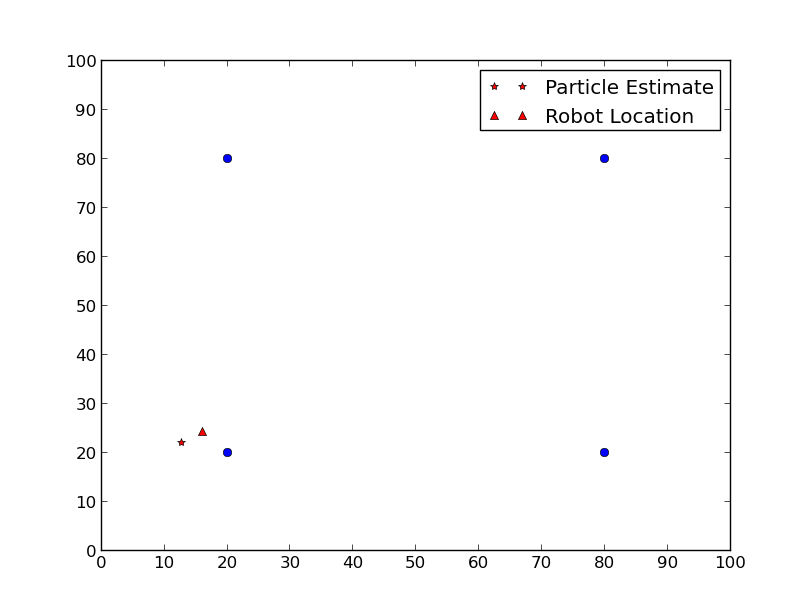
\includegraphics[width = 2.75 in]{2.png}}\qquad
  \subfigure[]{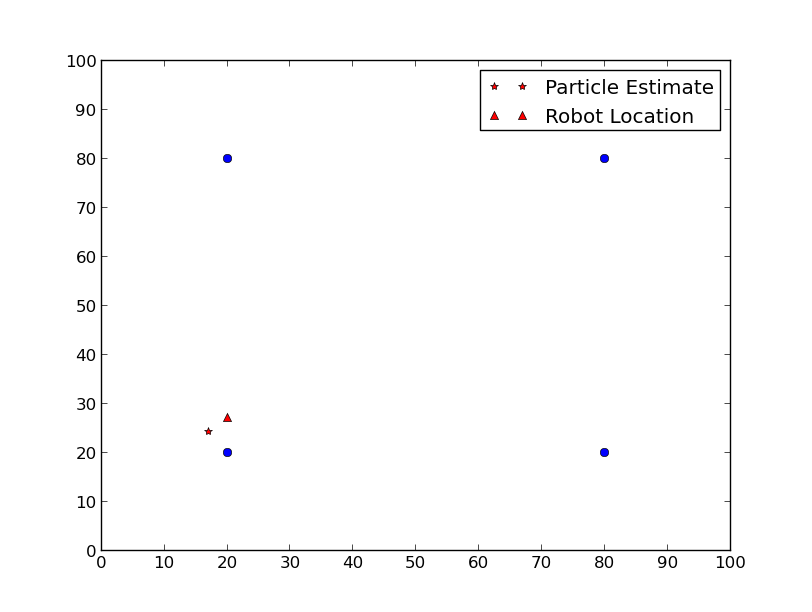
\includegraphics[width = 2.75 in]{3.png}}\qquad
  \subfigure[]{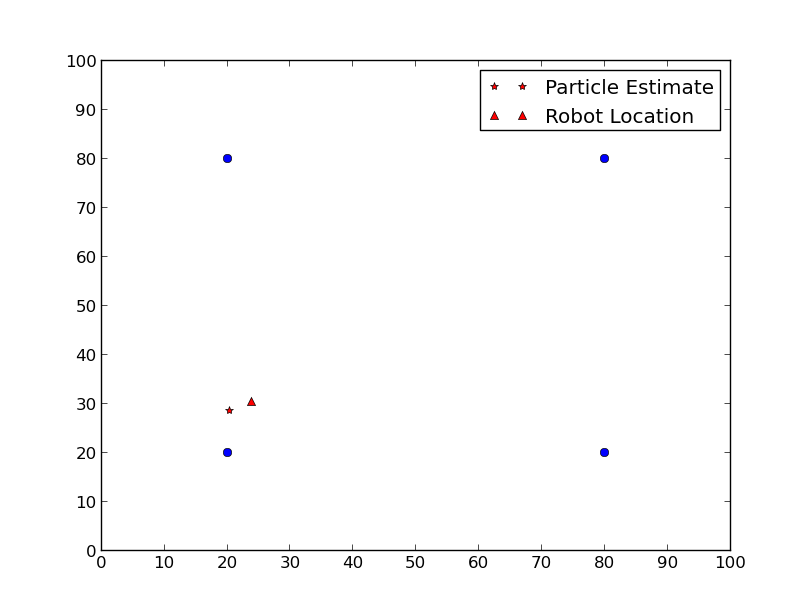
\includegraphics[width = 2.75 in]{4.png}}
  \caption{\label{fig-: movement simulation world}Particle Filters estimating the position of the robot
   The robot is moved at a constant velocity of 5 units/timestep in each case. The particle filters estimate the location of the robot (star) by integrating the motion and sensor models.}
\end{figure}



\section{Results}
In this section we describe the various experiments that were performed in our simulated world. To simulate changes in the envrionment I externally change the noise in robot's motion model. In the experiments external chagnes were simulated by artifically intoducting a drift in the motion, secondaly by changing the variance of the motion model distribution. The parameter estimation was based on smoothed trajectories therfore in the results we show how estimation of parameter varies with number of trajectories. As shown in Table ~\ref{tab-constant paramters} the total timesteps is 200 and in all the experiments we simulate the changes at time step 60. 

As desribed in Chapter ~\ref{chap-:Motion Model} the noise model for our simulated experiment is 

$V_{t}\sim\mathcal{{N}}(v_{t},v_{t}^{2}\sigma_{V_{v}}^{2}+w_{t}^{2}\sigma_{V_{w}}^{2}+\sigma_{V_{1}}^{2})$

$W_{t}\sim\mathcal{{N}}(w_{t},v_{t}^{2}\sigma_{w_{v}}^{2}+w_{t}^{2}\sigma_{V_{w}}^{2}+\sigma_{W_{1}}^{2})$

In first experiment we change $\sigma_{V_{v}}^2$ at time step 60 as shown in Table ~\ref{tab-:varying_sensor_noise}. The changed values of the parameter for first and second case are $0.5$ and $1.0$ respectively. The number of trajectories is 3 and is kept constant for both the cases. In this experiment we keep the sensor noise constant as well. 

\begin{table}[tbh]

\centering



\begin{tabular}{|c|c|c|c|c|c|c|c|}
\hline 
\multicolumn{2}{|c|}{Initial Parameter Values} & \multicolumn{2}{c|}{Changed Parameter Values (after 60)} & \multicolumn{2}{c|}{Estimated Parameter Values} & Sensor Noise & Trajectories\tabularnewline
\hline 
 &  & 1 & 2 & 1 & 2 &  & \tabularnewline
\hline 
$\sigma_{V_{v}}^{2}$ & 0.05 & 0.5 & 1.0 & 1.185 & 2.640 & 1.0 & 3\tabularnewline
\hline 
$\sigma_{V_{w}}^{2}$ & 0.05 & 0.05 & 0.05 & 0.05 & 0.05 & 1.0 & 3\tabularnewline
\hline 
$\sigma_{V_{1}}^{2}$ & 0.05 & 0.05 & 0.05 & 0.176 & 0.337 & 1.0 & 3\tabularnewline
\hline 
$\sigma_{W_{v}}^{2}$ & 0.05 & 0.05 & 0.05 & 0.05 & 0.05 & 1.0 & 3\tabularnewline
\hline 
$\sigma_{W_{v}}^{2}$ & 0.05 & 0.05 & 0.05 & 0.05 & 0.05 & 1.0 & 3\tabularnewline
\hline 
$\sigma_{W_{w}}^{2}$ & 0.05 & 0.05 & 0.05 & 0.05 & 0.05 & 1.0 & 3\tabularnewline
\hline 
$\sigma_{W_{1}}^{2}$ & 0.05 & 0.05 & 0.05 & 0.05 & 0.05 & 1.0 & 3\tabularnewline
\hline 
\end{tabular}
\caption{\label{tab-:varying_sensor_noise}Initial and estimated values of parameters with constant sensor noise
and trajectories}
\end{table}

As shown in Table ~\ref{tab-:varying_sensor_noise} the estimated value of $\sigma_{V_{v}}^2$ are $1.185$ and $2.640$ which are greater than the actual values and could lead to better localization. In order to demonstrate that I show the localization error i.e. euclidean error between the robot's actual position and location estimate of partilce filters. In Figure ~\ref{fig-varying_sensor_noise} the red and blue line shows the error with a static motion model and adaptive motion model respectively.

 
 
\begin{figure}
  \centering
     {\includegraphics[height = 3.0 in]{../../motion_model/plots/200_0.05_0.5_s_1_traj_3.eps}}
  \caption{\label{fig-varying_sensor_noise} }
\end{figure}
At the start of the experiment the parameter values for the robot's motion model and static motion model for particle filters are intialized with the same value. The adaptive motion model right from time step 0 starts estimating the parameters. In Figure ~\ref{fig-varying_sensor_noise} in the first $20$ there is no change and we can see that the adaptive motion model performs better than the static. In theory the static motion model has the best estimate of robot' motion as they are intialized with the same parameter value so the error should be less for static motion model. We don't see this because the location of particles are randomly initilazied therefore it might be at different location to robot's start position. It needs sensor model to decrease the error and as the sensor noise is high it takes time to build the weight of particles. In Figure ~\ref{varying_sensor_noise_sensor_model} we plot the average weight of particles at each time step and when the weights of particle are higher we can see the static motion model performing better. This is due to the resampling step of particle fitlers where they choose the most proabable particles based on motion and sensor models. As soon as the algorithm starts picking the most probabasle particles the error goes down and we can see that the average weight of particles are also higher. In the case of adaptive motion model the distribution of motion model gets wider right from the start and which leads to decrease in error.

After time step 60 we change the motion model noise and we can see that adative motion model performing way better as comparated to the static motion model. The average weight of partilces in Figure ~\ref{fig-varying_sensor_noise_sensor_model} also goes down. In Figure ~\ref{fig-varying_sensor_noise_motion_model} we don't see a jump in the red line or green line at time step 60 and this due to the fact that the estimate of parameter before the change was greater than the change after time step 60.   
   
\begin{figure}
  \centering
     {\includegraphics[height = 3.0 in]{../../motion_model/plots/200_0.05_0.5_s_1_traj_3_motion_model.eps}}
  \caption{\label{fig-varying_sensor_noise_motion_model} }
\end{figure}

\begin{figure}
  \centering
     {\includegraphics[height = 3.0 in]{../../motion_model/plots/200_0.05_0.5_s_1_traj_3_sensor_model.eps}}
  \caption{\label{fig-varying_sensor_noise_sensor_model} }
\end{figure}


\begin{table}[tbh]



\centering

\begin{tabular}{|c|c|c|c|c|c|c|c|c|c|}
\hline 
\multicolumn{2}{|c|}{Initial Parameter Values} & Changed Parameter Values & \multicolumn{3}{c|}{Estimated Parameter Values} & Sensor Noise & \multicolumn{3}{c}{Trajectories}\tabularnewline
\hline 
 &  & 1 & 1 & 2 & 3 &  &  &  & \tabularnewline
\hline 
$\sigma_{V_{v}}^{2}$ & 0.05 & 0.5 & 3.407 & 2.547 & 1.240 & 2.0 & 3 & 15 & 30\tabularnewline
\hline 
$\sigma_{V_{w}}^{2}$ & 0.05 & 0.05 & 0.05 & 0.05 & 0.05 & 2.0 & 3 & 15 & 30\tabularnewline
\hline 
$\sigma_{V_{1}}^{2}$ & 0.05 & 0.05 & 0.423 & 0.327 & 0.182 & 2.0 & 3 & 15 & 30\tabularnewline
\hline 
$\sigma_{W_{v}}^{2}$ & 0.05 & 0.05 & 0.05 & 0.05 & 0.05 & 2.0 & 3 & 15 & 30\tabularnewline
\hline 
$\sigma_{W_{v}}^{2}$ & 0.05 & 0.05 & 0.05 & 0.05 & 0.05 & 2.0 & 3 & 15 & 30\tabularnewline
\hline 
$\sigma_{W_{w}}^{2}$ & 0.05 & 0.05 & 0.05 & 0.05 & 0.05 & 2.0 & 3 & 15 & 30\tabularnewline
\hline 
$\sigma_{W_{1}}^{2}$ & 0.05 & 0.05 & 0.05 & 0.05 & 0.05 & 2.0 & 3 & 15 & 30\tabularnewline
\hline 
\end{tabular}
\caption{Initial and estimated values of parameters with varying trajectories}
\end{table}


\begin{table}[tbh]





\begin{tabular}{|c|c|c|c|c|c|c|c|c|c|}
\hline 
\multicolumn{2}{|c|}{Initial Parameter Values} & Changed Parameter Values & \multicolumn{3}{c|}{Estimated Parameter Values} & Sensor Noise & \multicolumn{3}{c}{Trajectories}\tabularnewline
\hline 
 &  & 1 & 1 & 2 & 3 &  &  &  & \tabularnewline
\hline 
$\sigma_{V_{v}}^{2}$ & 0.05 & 1.0 & 3.960 &  & 0.765 & 2.0 & 3 & 15 & 30\tabularnewline
\hline 
$\sigma_{V_{w}}^{2}$ & 0.05 & 0.05 & 0.05 & 0.05 & 0.05 & 2.0 & 3 & 15 & 30\tabularnewline
\hline 
$\sigma_{V_{1}}^{2}$ & 0.05 & 0.05 & 0.484 &  & 0.129 & 2.0 & 3 & 15 & 30\tabularnewline
\hline 
$\sigma_{W_{v}}^{2}$ & 0.05 & 0.05 & 0.05 & 0.05 & 0.05 & 2.0 & 3 & 15 & 30\tabularnewline
\hline 
$\sigma_{W_{v}}^{2}$ & 0.05 & 0.05 & 0.05 & 0.05 & 0.05 & 2.0 & 3 & 15 & 30\tabularnewline
\hline 
$\sigma_{W_{w}}^{2}$ & 0.05 & 0.05 & 0.05 & 0.05 & 0.05 & 2.0 & 3 & 15 & 30\tabularnewline
\hline 
$\sigma_{W_{1}}^{2}$ & 0.05 & 0.05 & 0.05 & 0.05 & 0.05 & 2.0 & 3 & 15 & 30\tabularnewline
\hline 
\end{tabular}
\end{table}


\begin{table}
\centering

\caption{Initial and estimated values of parameters with drift}


\begin{tabular}{|c|c|c|c|c|c|c|c|c|}
\hline 
\multicolumn{2}{|c|}{Initial Parameter Values} & Changed Parameter Values & \multicolumn{2}{c|}{Estimated Parameter Values} & \multicolumn{2}{c|}{Drift } & Trajectories & Sensor noise(after 60)\tabularnewline
\hline 
 &  & 1 & 1 & 2 & 1 & 2 &  & \tabularnewline
\hline 
$\sigma_{V_{v}}^{2}$ & 0.05 & 0.05 & 38.071 & 20.025 & 1.0 & 2.0 & 3 & 10.0\tabularnewline
\hline 
$\sigma_{V_{w}}^{2}$ & 0.05 & 0.05 & 0.05 & 0.05 & 1.0 & 2.0 & 3 & 10.0\tabularnewline
\hline 
$\sigma_{V_{1}}^{2}$ & 0.05 & 0.05 & 4.274 & 2.269 & 1.0 & 2.0 & 3 & 10.0\tabularnewline
\hline 
$\sigma_{W_{v}}^{2}$ & 0.05 & 0.05 & 0.05 & 0.05 & 1.0 & 2.0 & 3 & 10.0\tabularnewline
\hline 
$\sigma_{W_{v}}^{2}$ & 0.05 & 0.05 & 0.05 & 0.05 & 1.0 & 2.0 & 3 & 10.0\tabularnewline
\hline 
$\sigma_{W_{w}}^{2}$ & 0.05 & 0.05 & 0.05 & 0.05 & 1.0 & 2.0 & 3 & 10.0\tabularnewline
\hline 
$\sigma_{W_{1}}^{2}$ & 0.05 & 0.05 & 0.05 & 0.05 & 1.0 & 2.0 & 3 & 10.0\tabularnewline
\hline 
\end{tabular}
\caption{Initial and estimated values of parameters with varying trajectories}
\end{table}


\begin{table}[tbh]
\centering




\begin{tabular}{|c|c|c|c|c|c|c|c|c|c|c|}
\hline 
\multicolumn{2}{|c|}{Initial Parameter Values} & Changed Parameter Values & \multicolumn{3}{c|}{Estimated Parameter Values} & \multicolumn{1}{c|}{Drift } & \multicolumn{3}{c|}{Trajectories} & Sensor noise(after 60)\tabularnewline
\hline 
 &  &  & 1 & 2 & 3 &  & 1 & 2 & 3 & \tabularnewline
\hline 
$\sigma_{V_{v}}^{2}$ & 0.05 & 0.05 & 20.025 & 0.713 & 0.569 & 2.0 & 3 & 15 & 30 & 10.0\tabularnewline
\hline 
$\sigma_{V_{w}}^{2}$ & 0.05 & 0.05 & 0.05 & 0.05 & 0.05 & 2.0 & 3 & 15 & 30 & 10.0\tabularnewline
\hline 
$\sigma_{V_{1}}^{2}$ & 0.05 & 0.05 & 2.269 & 0.123 & 0.107 & 2.0 & 3 & 15 & 30 & 10.0\tabularnewline
\hline 
$\sigma_{W_{v}}^{2}$ & 0.05 & 0.05 & 0.05 & 0.05 & 0.05 & 2.0 & 3 & 15 & 30 & 10.0\tabularnewline
\hline 
$\sigma_{W_{v}}^{2}$ & 0.05 & 0.05 & 0.05 & 0.05 & 0.05 & 2.0 & 3 & 15 & 30 & 10.0\tabularnewline
\hline 
$\sigma_{W_{w}}^{2}$ & 0.05 & 0.05 & 0.05 & 0.05 & 0.05 & 2.0 & 3 & 15 & 30 & 10.0\tabularnewline
\hline 
$\sigma_{W_{1}}^{2}$ & 0.05 & 0.05 & 0.05 & 0.05 & 0.05 & 2.0 & 3 & 15 & 30 & 10.0\tabularnewline
\hline 
\end{tabular}
\caption{Inital and estimated values of parameters with drift and varying trajectories}
\end{table}

 
\chapter{Landmarks extraction using Side Sonar Images}
\section{Introduction}
\subsection{Side Scan Sonar} 
\subsection{Speeded Up Robust Features}

\section{Dynamic Landmarks}
In the particle filtering algorithm the sensor model is responsible to assign weights to the particles.The sensor model describes the process by which sensor measurements are generated in the physical world.It is generally done by using some sort of references in the world aka landmarks. Austin and Elizar in their papers used static maps of known environments to generate references for their sensor model.
The probability of having static maps for underwater environments is pretty low and thus lead us to use side sonar images as references for the sensor model.
\begin{figure}[hbtp]
\caption{Side Sonar Image}
\centering
\includegraphics[scale=0.5]{/home/rohan/Documents/thesis_work/visual_sonar/sonar_59/18.jpg}
\end{figure}
As you can see in the image there are lot of horizontal lines which we treat as noise. For us to use the side sonar images we performed a pre-processing step in which we used a median filter on the image. This helped us in getting rid of major noises in terms of horizontal lines but also blurred the image. In order to generate some landmarks we ran feature extractions techniques like SURF. This algorithm helped us in detecting interest points in the image and are shown below in circles. Andrew Vardy{refer the paper) ran multiple image registration techniques such as phase matching (you need to mention more) on side sonar images and showed that SURF performs better than the rest .
\begin{figure}[hbtp]
\caption{SURF Keypoints}
\centering
\includegraphics[scale=0.4]{/home/rohan/Documents/thesis_work/visual_sonar/landmarks.png}
\end{figure}

These interest points can be treated as landmarks. We use a high Hessian
threshold so that we have a maximum of 4 landmarks. The distance of the robot and the particles to these landmarks are used to assign weights to the particles.
\\
The output of a side sonar is a ping of the surface and for an image to be created we need to combine pings over time. Andrew Vardy in his paper explains on how to combine pings to create an meaningful image. For our algorithm to run on the AUV we can use Andrew's algorithm as a black box and run our feature extraction on the output i.e. images of the seabed. 
This method allows us independence from a static map as well as helps in learning
the motion model on the fly in a new environment. 

\section{Motion Estimation using side sonar images}
In AUV the motion estimation is generally done through dead-reckoning.
It is a process of calculating the current position based upon the
previous position and the speed of vessel. The velocity of the AUV
can be estimated by the acceleration measurement supplied by an Inertial
Measurement Unit. Another way is to use a Doppler Velocity Log(DVL) that
measures velocity in water by measuring the Doppler effect on scattered
sound waves. Dead reckoning may have significant errors as the velocity
and direction must be accurately known at every time step. 

In this algorithm we propose to get motion estimates using side sonar
images. As stated before we run SURF on the images and generate some
key points. These key points are matched in the next image using a
KNN based matcher. The matched key points gives us an estimate on
the movement of the vehicle. In the figure we show two consecutive
images and in the first image we have the key points marked in circle.
In the next image we have the matched key points marked in green circles. 
\begin{figure}[hbtp]
\caption{SURF Keypoints}
\centering
\includegraphics[scale=0.4]{/home/rohan/Documents/thesis_work/visual_sonar/surf_working.jpeg}
\end{figure}
This estimate can be coupled with the previous estimate to calculate
the current position. The visual input to the dead reckoning algorithm
has its pros and cons.The main advantage of using a visual estimate
is that it doesn't suffer from drift which is prime concern for underwater
vehicles. The disadvantage lies in the fact that we don't have side
sonar images available every time. We can solve the problem by combining
the visual input with the velocity estimates. We can pass the visual
motion estimate and the DVL estimate to a Kalman Filter and use the
output as an input to our dead-reckoning estimate. The second disadvantage
is the computation power available on AUV. To specifically deal with
the problems we use a high Hessian threshold to extract maximum of
4 landmarks so that feature matching is not computationally expensive. 

We validate our algorithm on datasets consisting of side sonar images
and the total distance the AUV moves. 


\chapter{Results}
\section{Adapting Motion Model}
\label{results}
We use a simulation to demonstrate the effectiveness of learning the
motion model. The simulation mainly consists of particle filter SLAM.
We use a motion model described in the above chapters. The sensor
model basically measures the distance from the four static landmarks
defined at the start of the experiment. The experiment runs over 100
time steps and at every 5\textsuperscript{th} time step we change
the parameters of the motion model. As described in the above chapters
the parameters that we intended to learn are $\sigma_{D_{d}}^{2}$,$\sigma_{T_{d}}^{2}$,$\sigma_{D_{1}}^{2},\sigma_{D_{r}}^{2}$,$\sigma_{T_{r}}^{2}$,$\sigma_{D_{1}}^{2}$,$\sigma_{T_{1}}^{2}$.
In the first stage of the experiment at every 5\textsuperscript{th }time step
we change $\sigma_{D_{d}}^{2}$ or $\sigma_{T_{r}}^{2}$in our motion
model. The following table and plots describes the five experiments
that were conducted in the simulation.

\begin{tabular}{|c|c|c|c|c|c|}
\hline 
No. & $\sigma_{D_{d}}$ & $\sigma_{T_{r}}$ & $\sigma_{D_{d}}^{*}$ & $\sigma_{T_{r}}^{*}$ & Sensor Noise\tabularnewline
\hline 
\hline 
1 & 0.05 & 0.05 & 0.2 & 0.05 & 2.0\tabularnewline
\hline 
2 & 0.05 & 0.05 & 0.2 & 0.05 & 5.0\tabularnewline
\hline 
4 & 0.05 & 0.05 & 0.5 & 0.05 & 2.0\tabularnewline
\hline 
5 & 0.05 & 0.05 & 0.5 & 0.05 & 5.0\tabularnewline
\hline 
6 & 0.05 & 0.05 & 0.05 & 0.2 & 5.0\tabularnewline
\hline 
7 & 0.05 & 0.05 & 0.05 & 0.5 & 5.0\tabularnewline
\hline 
\end{tabular}
\\

$\sigma_{D_{d}}$,$\sigma_{T_{r}}$ are the parameters values that
the motion model was initialized. These values are altered in order
to simulate a change in the motion model and they are described by
$\sigma_{D_{d}}^{*}$,$\sigma_{T_{r}}^{*}$. The sensor noise can
be described as the confidence the robot has in its sensor model .
The impact of the noise on the localization error can be seen in the
following plots.	

\begin{figure}
\caption{$\sigma_{D_{d}}$=0.05 $\sigma_{D_{d}}^{*}$ = 0.2 Sensor Noise= 2.0}


\includegraphics[scale=0.25]{\lyxdot \lyxdot /plot_motion_model/100_0\lyxdot 05_0\lyxdot 2_1_2\lyxdot 0_motion_model_1}
\end{figure}


\begin{figure}
\caption{$\sigma_{D_{d}}$=0.05 $\sigma_{D_{d}}^{*}$ = 0.2 Sensor Noise= 5.0}


\includegraphics[scale=0.25]{\lyxdot \lyxdot /plot_motion_model/100_0\lyxdot 05_0\lyxdot 2_1_5\lyxdot 0_motion_model_1}

\end{figure}


Figure 1 and Figure 2 are plots of the localization error with different
sensor noises. We can see in both the cases the learned motion model
performed better than the static motion model. Another important point
is that the average error is less when the sensor noise is 2.0 as
compared to the second case. This can be accounted for the fact that
our localization algorithm is more confident on the sensor model as
compared to the motion model. 

\begin{figure}
\caption{$\sigma_{D_{d}}$=0.05 $\sigma_{D_{d}}^{*}$ = 0.5 Sensor Noise= 2.0}


\includegraphics[scale=0.25]{\lyxdot \lyxdot /plot_motion_model/100_0\lyxdot 05_0\lyxdot 5_1_2\lyxdot 0_motion_model}

\end{figure}


\begin{figure}
\caption{$\sigma_{D_{d}}$=0.05 $\sigma_{D_{d}}^{*}$ = 0.5 Sensor Noise= 5.0}


\includegraphics[scale=0.25]{\lyxdot \lyxdot /plot_motion_model/100_0\lyxdot 05_0\lyxdot 5_1_5\lyxdot 0_motion_model_1}

\end{figure}


As we can see in Figure 3 and Figure 4 at 5\textsuperscript{th} time
step the error shooting up but the learned motion model brings back
the error whereas the static motion model takes time to recover back
depending upon the sensor noise. In both the figures we can see that
the error is pretty static in the learned motion model whereas in
the static motion model there is a lot of fluctulation. 

\begin{figure}
\caption{$\sigma_{T_{r}}$=0.05 $\sigma_{T_{r}}^{*}$ = 0.2 Sensor Noise= 5.0}


\includegraphics[scale=0.75]{\lyxdot \lyxdot /plot_motion_model/100_0\lyxdot 05_0\lyxdot 2_rotation_5\lyxdot 0_motion_model}

\end{figure}


\begin{figure}
\caption{$\sigma_{T_{r}}$=0.05 $\sigma_{T_{r}}^{*}$ = 0.5 Sensor Noise= 5.0}


\includegraphics[scale=0.25]{\lyxdot \lyxdot /plot_motion_model/100_0\lyxdot 05_0\lyxdot 5_rotation_5\lyxdot 0_motion_model}

\end{figure}


Figure 5 and Figure 6 describe the errors when the robot rotational
motion is much more than the translational motion. We can clearly
see that the learned motion model quickly adapts to the changes whereas
the static motion model struggles to get the error down. 

In all the cases it was very clear that we could see the adaptive
motion model performing better than the static. The sensor noise had
its impact on the overall error. Robot calibration is important to
process in mobile robotics. The proposed algorithm is an automated
process which can help us in better navigation of the robots and can
be used for any motion model. 
\section{Motion estimation using side sonar images}

\chapter{Conclusion}

Did it!

\bibliographystyle{plain}
\bibliography{mendeley.bib}

\end{document}
